\documentclass[12pt]{article}
\usepackage[utf8]{inputenc}
\usepackage[T1]{fontenc}
\usepackage{svg}
\usepackage{amsmath}
\usepackage{lastpage}
\usepackage{hyperref}
\usepackage{listings}
\usepackage{xcolor}
\usepackage{booktabs} % For prettier tables
\usepackage{multicol}
\usepackage{multirow}
\usepackage[shortlabels]{enumitem}
\usepackage{hyperref}
\usepackage{cleveref}
\usepackage{subcaption}
\usepackage{fancyhdr}
\usepackage[colorinlistoftodos]{todonotes}
\usepackage[numbers,sort&compress]{natbib}
\usepackage{graphicx}
\usepackage{pdflscape}
\graphicspath{ {./Figures/} {./diagrams/} {./plots/} } % Sets asset lookup paths



% --- Draft comment layout (doesn't change the main text width) ---
\setlength{\marginparwidth}{4.6cm} % try 3cm, 4cm, 5cm...
\setlength{\marginparsep}{-1cm}
%\usepackage[textwidth=\marginparwidth]{todonotes}
% NICE HIGHLIGHT OF COMMENTED TEXT
\usepackage{soul} % provides \texthl

\makeatletter
\if@todonotes@disabled
  \newcommand{\hlfix}[2]{#1}
\else
  \newcommand{\hlfix}[2]{#1\todo{#2}}
\fi
\makeatother



\usepackage{array}
\usepackage{ragged2e}
\usepackage{multirow}
\newcolumntype{P}[1]{>{\centering\arraybackslash}p{#1}} % center the column and justify its contents to the top in multirow tables
\newcolumntype{R}[1]{>{\RaggedLeft\arraybackslash}p{#1}} % Align column to the right in multirow tables

\definecolor{codegreen}{rgb}{0,0.6,0}
\definecolor{codegray}{rgb}{0.5,0.5,0.5}
\definecolor{codepurple}{rgb}{0.58,0,0.82}
\definecolor{backcolour}{rgb}{0.95,0.95,0.92}

\lstdefinestyle{mystyle}{
    backgroundcolor=\color{backcolour},   
    commentstyle=\color{codegreen},
    keywordstyle=\color{magenta},
    numberstyle=\tiny\color{codegray},
    stringstyle=\color{codepurple},
    basicstyle=\ttfamily\footnotesize,
    breakatwhitespace=false,         
    breaklines=true,                 
    captionpos=b,                    
    keepspaces=true,                 
    numbers=left,                    
    numbersep=5pt,                  
    showspaces=false,                
    showstringspaces=false,
    showtabs=false,                  
    tabsize=2
}

\lstset{style=mystyle}

% --- set footer and header ---
\renewcommand{\headrulewidth}{1pt}
\renewcommand{\footrulewidth}{1pt}
\title{Title}
\pagestyle{fancy}
\fancyhf{}

\makeatletter\let\Title\@title\makeatother

\lhead{\Title}
\rfoot{\includegraphics[height=1cm]{Figures/logo_small.png}} % right header logo
\setlength\headheight{16pt}
\setlength{\footskip}{50pt}
\lhead{\Title} %rightH title
\cfoot{\thepage}
% --- end footer and header ---

%----------EDIT COVER INFO HERE -----------------%

\def \LOGOPATH {Figures/ITU.svg}
\def \DEPARTEMENT {Department of Computer Science}
\def \COURSENUM {KISPECI1SE}
\def \COURSENAME {Master Thesis}
\def \REPORTTITLE {The Deflective Advantage: Reducing Impact Shock and Vibration in Confined-Space Drone Operations}
\def \STUDENTNAME {Jakub Sejkora (jsej@itu.dk)}
\def \INSTRUCTOR {Alejandro Lorite Mora}

%------------------------------------------------%

\begin{document}

\hypersetup{pageanchor=false}

\pagenumbering{Roman}

\begin{titlepage}
    \vfill
    \begin{center}
    \includegraphics[width=0.7\textwidth]{Figures/logo_small.png} \\
        \hfill \\
        \Large{\DEPARTEMENT} \\
        \Large{\COURSENUM\;-\;\COURSENAME} \\
        \vfill
        \textbf{\LARGE{\REPORTTITLE}}
    \end{center}
    \vfill
    \begin{flushleft}
        \Large{\textbf{Prepared by:} \STUDENTNAME} \\
        \Large{\textbf{Supervised by:} \INSTRUCTOR} \\
        \Large{\textbf{Date:} \today}
    \end{flushleft}
    \vfill
\end{titlepage}

%-----------------------------------------------%

%\tableofcontents
%\clearpage



\begin{abstract}

This thesis investigates whether a mechanical deflection mechanism---a freely rotating protective cage---can reduce impact shock and vibration in confined-space drone operations, and whether the onboard inertial signatures of those collisions can be exploited for spatial awareness.

A custom 4-inch autonomous quadcopter was designed and built, integrating a Pixhawk~6C flight controller running PX4, a Raspberry~Pi~5 companion computer running ROS~2, and a PETG spherical cage (35.8\,cm diameter) tested in two configurations: rigidly fixed and bearing-decoupled (freely rotating). All other parameters---mass, diameter, material, and propeller clearance---were held constant, isolating the bearing mechanism as the single independent variable. Experiments were conducted in an OptiTrack motion-capture environment, with the drone executing 179 autonomous collision passes against a static cylindrical obstacle at approach angles of $45^\circ$ and $75^\circ$. After telemetry-based verification, 127 structural impacts were isolated for comparative analysis.

The rotating cage reduced maximum impact deceleration by 59\% relative to the fixed configuration ($-1.64 \pm 0.64$\,m/s$^2$ vs.\ $-1.03 \pm 0.50$\,m/s$^2$, $p < 0.001$, Cohen's $d = 1.05$), and IMU vibration analysis revealed a narrower post-impact oscillation envelope with faster return to the nominal noise floor. The bearing mechanism introduced a modest spatial trade-off: maximum trajectory deviation increased slightly (Fixed: $118.4 \pm 30.4$\,mm; Rotating: $131.0 \pm 32.1$\,mm, $p = 0.022$, $d = 0.41$), but the total recovery area remained statistically indistinguishable ($p = 0.998$), indicating that the flight controller's PID correction capacity absorbed the offset.

To evaluate whether impact angle can be inferred from onboard sensors alone, a Random Forest regressor was trained on 14 IMU-derived features. Cross-validated $R^2$ reached approximately 0.72 for both configurations, with mean absolute error of $4.5^\circ$--$4.9^\circ$---sufficient to distinguish glancing from deeper collisions. Critically, the rotating cage's angle signature was invisible to linear models (Huber baseline $R^2 = 0.004$) yet fully recovered by the non-linear Random Forest ($R^2 = 0.719$), and cross-condition transfer between cage types failed decisively ($R^2 < 0.26$), demonstrating that the bearing mechanism fundamentally redistributes---rather than destroys---the angle information carried by the vibration signature.

These findings establish the rotating cage as an effective mechanical countermeasure for impact survivability and open the door to \emph{tactile SLAM}: navigation by contact in environments where no other sensor modality is viable.

\end{abstract}

\hypersetup{pageanchor=true}

\newpage

\tableofcontents

\newpage
\pagenumbering{arabic}
\fancyfoot[C]{Page \thepage\ of \pageref{LastPage}}
\section*{Table of Acronyms}
\addcontentsline{toc}{section}{Table of Acronyms}

\begin{table}[htbp]
\centering
\begin{tabular}{p{0.22\textwidth}p{0.68\textwidth}}
\toprule
\textbf{Acronym} & \textbf{Definition} \\
\midrule
ARQ & Actively Resilient Quadrotor \\
BSD & Berkeley Software Distribution (open-source license) \\
EKF & Extended Kalman Filter \\
ENU & East-North-Up (coordinate frame) \\
ESC & Electronic Speed Controller \\
FRD & Forward-Right-Down (coordinate frame) \\
GPL & General Public License \\
IMU & Inertial Measurement Unit \\
LiDAR & Light Detection and Ranging \\
MAE & Mean Absolute Error \\
MAVLink & Micro Air Vehicle Link (communication protocol) \\
MCAP & Message Capture (ROS 2 logging format) \\
MoCap & Motion Capture \\
NED & North-East-Down (coordinate frame) \\
PETG & Polyethylene Terephthalate Glycol (3D printing filament) \\
PID & Proportional-Integral-Derivative (control algorithm) \\
PX4 & Pixhawk Autopilot Firmware v4 \\
$R^2$ & Coefficient of Determination \\
RMSE & Root Mean Square Error \\
ROS 2 & Robot Operating System 2 \\
RPM & Revolutions Per Minute \\
RTOS & Real-Time Operating System \\
SIAE & Spatial Integral of Absolute Error \\
SITL & Software-in-the-Loop (simulation) \\
SLAM & Simultaneous Localization and Mapping \\
TWR & Thrust-to-Weight Ratio \\
UART & Universal Asynchronous Receiver-Transmitter \\
UAV & Unmanned Aerial Vehicle \\
uORB & micro Object Request Broker (PX4 middleware) \\
uXRCE-DDS & micro XRCE-DDS (PX4-ROS 2 bridge protocol) \\
VIO & Visual-Inertial Odometry \\
WP & Waypoint \\
\bottomrule
\end{tabular}
\end{table}

\newpage
\clearpage
\section{Introduction}

\textbf{Aerial Inspection in Confined Spaces.}
The deployment of Unmanned Aerial Vehicles (UAVs) has significantly advanced the field of industrial inspection. In expansive, outdoor environments, drones are now routinely utilized to inspect power lines, bridge infrastructure, and wind turbines, drastically reducing the risk to human operators while increasing efficiency. However, the transition of autonomous aerial robotics into indoor, confined spaces remains a significant challenge. Industries rely heavily on complex internal structures---such as large-scale storage vats, subterranean networks, and industrial piping---that require frequent inspection. Yet, the adoption of autonomous UAVs in these spaces severely lags behind outdoor applications due to a severe set of environmental constraints \cite{ozaslan2017inspection}.

\textbf{Navigation Challenges in GPS-Denied Environments.}
Operating a UAV within confined industrial spaces, such as a stainless steel storage tank, fundamentally alters the requirements for flight. These environments are routinely GPS-denied and, due to heavy ferromagnetism or physical shielding, completely signal-denied. This severs the link to human pilots, mandating full onboard autonomy. However, achieving autonomy in these conditions exposes the limitations of standard sensor suites. Featureless or highly reflective surfaces confound optical cameras, while traditional 3D LiDAR systems are often too heavy for the payload capacity of a drone small enough to enter the space \cite{khattak2020robust}. Furthermore, even if the sensors could accurately map the environment, poses a substantial computational burden---a challenge that even ground-based autonomous vehicles struggle to solve reliably in much simpler 2D environments \cite{macariorojas2021}.

\textbf{Collision Resilience as a Navigation Modality.}
Given the strict payload limits on onboard companion computers and the unreliability of traditional sensors in hostile environments, complex, real-time collision avoidance becomes computationally impractical. In tight spaces, collisions are not a symptom of system failure; they are an inevitability. Therefore, the paradigm of autonomous confined-space flight must shift from attempting to avoid obstacles at all costs to surviving them and, ultimately, exploiting them.

Surviving these inevitable impacts requires a mechanical design capable of significantly lowering the kinetic penalty of a collision. This could perhaps be achieved by a structural design that, to a certain extent, deflects the collision forces away from the drone's main frame. While commercial solutions addressing this exist---such as the Flyability Elios \cite{briod2014collision}, which utilizes a freely rotating cage to roll along surfaces---empirical flight data detailing their performance during impact events remain sparse in the open literature---a gap that must be investigated before physical impacts can be reliably exploited for navigation.

\textbf{Research Objectives.}
If physical collisions in signal-denied environments are inevitable, and if a UAV can be designed to reliably survive them, a new avenue for spatial perception emerges. Rather than relying on heavy optical or laser-based sensors, a drone could theoretically utilize the very impacts it sustains to understand its surroundings. By interpreting the raw inertial data generated at the moment of collision, an autonomous system could extract foundational geometric information about its environment. If a drone operating without an external localization system can estimate the geometric angle of an impact using only its IMU, it gains a form of ``tactile odometry.'' Successive collisions could allow the system to map the boundaries of a confined space purely by bouncing off them. This transition---from a drone that is merely blind and resilient to one that is blind but tactile---forms the core of this investigation.

\subsection{Research Questions}

To address the need to deflect impact forces and redirect linear momentum, and to investigate the potential for collision exploitation, this thesis details the physical and software development of a custom, autonomous quadcopter equipped with an onboard companion computer and a freely rotating protective cage. By mechanically decoupling the protective outer shell from the drone's main frame, this design introduces a mechanism to redirect linear momentum into cage rotation, mitigating the impact penalty transferred to the airframe.

Using a ground truth motion capture (MoCap) environment to validate the system, this research seeks to answer the following questions:

\begin{enumerate}
    \item How does the physical resilience and energy deflection capability of a freely rotating protective cage compare to a fixed cage during direct obstacle collisions?
    \item To what extent can the raw inertial data generated during these deliberate physical collisions be utilized to accurately estimate the angle of impact against an obstacle, serving as a fundamental step toward tactile spatial awareness in signal-denied environments?
\end{enumerate}

\clearpage
\section{Related Work}

\subsection{Navigation by Contact and Tactile SLAM}

In highly cluttered or signal-denied environments, traditional collision-avoidance algorithms demand significant computational overhead and rely on heavy optical or LiDAR sensors that frequently fail in feature-poor spaces. While Simultaneous Localization and Mapping (SLAM) remains an active research frontier, reliably deploying it on small, payload-constrained drones in unstructured environments remains an open challenge~\cite{macariorojas2021}. Even state-of-the-art autonomous ground vehicles equipped with expensive sensors and substantial compute have not fully solved reliable real-time navigation in arbitrary environments; the task is substantially harder for a small aerial vehicle.

The constraint of navigating these spaces safely motivates a fundamentally different approach. Mulgaonkar et al.~\cite{mulgaonkarRobustAerialRobot2018} demonstrated that swarms of 25\,g micro-drones could navigate blind environments by intentionally colliding with obstacles and recovering from the impact, rather than detecting and avoiding them. This inverts the traditional SLAM paradigm: instead of building a map to avoid obstacles, the environment is explored through physical contact.

Furthermore, the ability to estimate contact state and impact forces using onboard odometry---termed \emph{contact-inertial odometry}---has been demonstrated to sustain state estimation during collisions by generating pseudo-measurements from external force estimates~\cite{de_petris_collision_2022}. This capability is directly relevant to aerial physical interaction and manipulation (APhI), where Reinforcement Learning (RL) policies must contend with contact dynamics that are difficult to model mathematically, complicating the construction of realistic training environments and reward functions~\cite{borgherini_oneshot_2025}. Recent work has attempted to bridge this gap via inner-loop dynamics estimators that compensate for unmodeled interaction forces within the RL framework~\cite{singh_reinforcement_2026}, underscoring the need for accurate force-feedback estimates of the kind that contact-inertial odometry can provide.

\subsection{Collision-Resilient Drone Designs}

Scaling this collision-resilience concept from 25\,g disposable swarms to a platform capable of carrying inspection sensors and a companion computer introduces a size-dependent penalty. At the 4-inch propeller class, the ratio of inertia to structural strength decreases, and obstacles that a micro-drone's simple tube cage could deflect become proportionally larger relative to the airframe. The protective cage must shield the propellers and fuselage from corners, shelves, and continuous piping---geometries that a minimal cage cannot deflect.

To manage this kinetic penalty, a significant portion of the literature has focused on energy absorption through structural compliance, utilising tensegrity structures~\cite{zhaDesignControlCollisionresilient2023}, arthropod-inspired elastic exoskeletons~\cite{azambujaWhenBeingSoft2022}, and shape-memory origami guards~\cite{parkOrigamiKirigamiStructure2023}. However, these compliant designs often introduce aerodynamic instability or scale poorly to standard industrial inspection platforms.

A more mechanically straightforward approach involves rigid, protective cages that physically decouple the drone's attitude from the collision surface. To ensure self-righting after ground impacts, Mulgaonkar et al.~\cite{mulgaonkarRobustAerialRobot2018} utilised G\"omb\"oc-shaped shells---a convex mono-monostatic body with a single stable equilibrium---for their 25\,g micro-drone swarms. Separately, Mahmud~\cite{mahmudDevelopmentCollisionResilient2021} explored rotating-shell principles, comparing a truncated icosahedron cage on a 3-axis gimbal against a simpler, single-axis turtle-shell cage; he concluded the truncated icosahedron was \emph{more efficient in minimising collision forces for all possible oblique collisions}, while the turtle-shell was the better choice only when low cost and reduced complexity were paramount. Both designs were successfully able to reorient into a take-off position after a crash.

\begin{figure}[htbp]
    \centering
    \begin{subfigure}{0.48\textwidth}
        \centering
        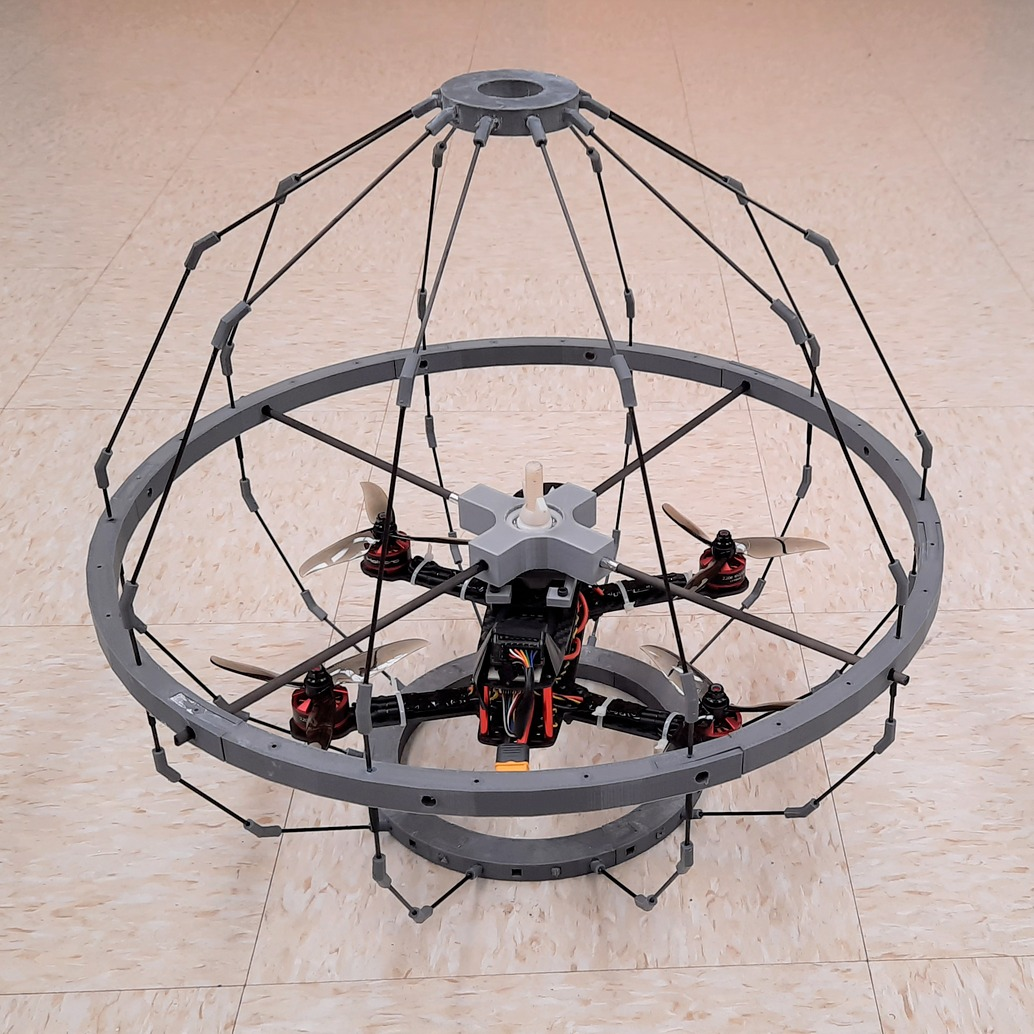
\includegraphics[width=\textwidth,height=4.5cm,keepaspectratio]{Figures/mahmud_turtle_cage.jpg}
        \caption{Mahmud's turtle-shell cage design. Adapted from~\cite{mahmudDevelopmentCollisionResilient2021}.}
        \label{fig:mahmud_turtle}
    \end{subfigure}
    \hfill
    \begin{subfigure}{0.48\textwidth}
        \centering
        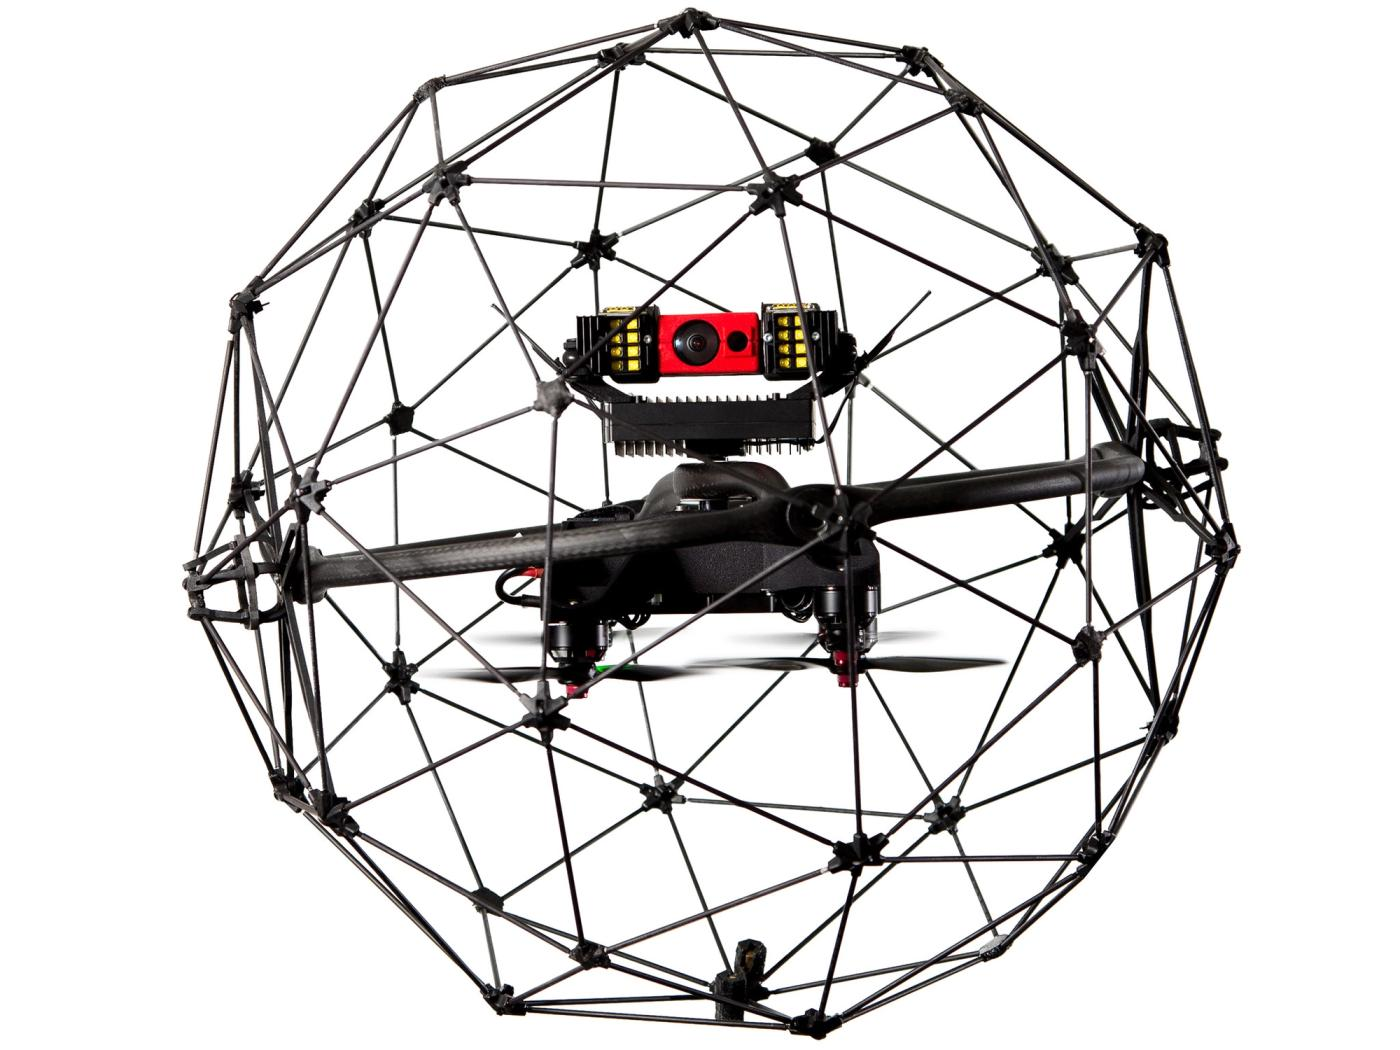
\includegraphics[width=\textwidth,height=4.5cm,keepaspectratio]{Figures/Elios_Flyability.jpg}
        \caption{Flyability Elios 3 inspection drone. Image: flyability.com.}
        \label{fig:elios}
    \end{subfigure}
    \caption{Collision-resilient cage designs in research and industry. (a)~Mahmud's single-axis turtle-shell cage demonstrating the rotating-shell principle; (b)~the commercially deployed Flyability Elios series confirming the practical viability of decoupled protective cages.}
    \label{fig:cage_designs}
\end{figure}

The rotating-cage concept has also reached commercial maturity in the Flyability Elios series~\cite{briod2014collision}, confirming the practical viability of decoupled protective cages for confined-space inspection.

Freely rotating spherical cages provide a distinct kinematic advantage during the \emph{airborne} impact itself: they convert linear collision momentum into rotational energy. This mechanism allows the cage to roll along a surface rather than scrape, mitigating the aggressive stick-slip friction dynamics that typically destabilise a drone's flight controller during sustained contact. This principle of kinetic impact deflection forms the mechanical baseline investigated in this thesis.

\subsection{Tactile Sensing and the IMU Noise Problem}

The concept of using physical contact as a sensing modality has precedent in robotics literature. In ground robotics, tactile whiskers and force-sensitive skins have long been used to map environments in low-visibility conditions. Extending this to aerial vehicles, the challenge is that contact events are highly transient and high-bandwidth, demanding both mechanical resilience to survive the impact and sufficient sensor fidelity to record meaningful data through the shock.

Currently, extracting this information from standard onboard sensors remains an open challenge. The dominant assumption in the literature is that standard commercial Inertial Measurement Units (IMUs) are unsuitable for accurate impact characterisation. Liu and Karydis~\cite{liuImpactresilientQuadrotorDesign2021} explicitly noted that the transient shockwaves of a collision overwhelm standard IMUs, rendering the data too noisy for reliable state estimation. To bypass this limitation, they equipped their Actively Resilient Quadrotor (ARQ) with custom Hall sensors mounted on prismatic shock absorbers to measure impact forces mechanically.

The combination of a deflection mechanism with onboard inertial measurement for angle inference, as pursued in this work, represents a novel intersection of these requirements. While traditional linear filtering struggles to extract meaningful collision geometry from chaotic IMU data, the noise generated by an impact is structurally dictated by the drone's collision mechanics. By applying a non-linear Random Forest regressor to these vibrational signatures, this thesis investigates whether the impact angle can be mathematically decoded from standard IMU data alone, potentially eliminating the need for specialised contact sensors in confined-space operations.

\section{Methodology}
\label{sec:methodology}
The methodology for this thesis project stands on the development of a drone to use for the various tests and implementations, together with a controlled environment to test the drone in.
The development consists of hardware choices, software choices, and the constraints arising from these two, which dictate much of the design. 
\subsection{Design and Development}
\subsubsection{Flight Type}
A quadcopter design was a very clear choice as these are widely used and allow for very nimble and precise movement as opposed to fixed-wing designs which need to be in forward motion to generate upthrust for their flight. The Quadcopter design due to its symmetric nature make it very easy to predictably control it. 

On figure \autoref{fig:drone_movement} you can see standard quadcopter setup. If front motors ($m_1$, $m_2$) spin comparatively more the drone pitches up, if side propelers ( $m_1$, $m_4$) spin comparatively faster, then the drone rolls towards its left side, and thanks to the setup of alternating spin direction if propellers diagonally from each other fx $m_1$ and $m_3$ will spin faster, while $m_2$ and $m_4$ will spin slower the drone will turn on around in the direction of the propolers which are faster, in this case turn towards its left. This is given by Newton's first law as the inertia of propellers spinning faster will induce the rotation in the propellers' direction.
Opposingly, pitch and roll is achieved by spinning pairs of propellers on one side faster than on the other (left vs right, front vs back).
This makes the control of quadcopter somewhat simple as it can be summarized in a mathematical model.
\begin{figure}
    \centering
    \includegraphics[width=1\linewidth]{Figures/drone_movement_pareto.png}
    \caption{typical quadrocopter setup 'props-in', yaw $\psi$ (turning around), pitch $\theta$ (nose up or down) and roll $\phi$ (tilting to sides) From \cite{gomezParetoOptimalPID2020}}
    \label{fig:drone_movement}
\end{figure}
\subsubsection{Constraints and Design Objectives}
This work is a continuation of the Spinfly platform by A.~Lerche \cite{lercheSpinFlyUAVSystem}, which identified two primary limitations that directly shaped this project: \textbf{insufficient weight headroom}---the original platform struggled with takeoff when equipped with the protective cage, leaving no margin for component upgrades---and \textbf{insufficient battery capacity}, which created operational friction by limiting test throughput.

These problems are coupled: battery mass scales with capacity, yet a heavier battery forces higher motor output, accelerating discharge and potentially negating the added capacity. Solving both simultaneously required systematic trade-off analysis. Lerche also noted a lack of robust autonomous control and unreliable telemetry, which informed the autopilot selection.

From these constraints, three design targets were formulated:
\begin{enumerate}
    \item \textbf{Carry larger payloads} --- sufficient headroom for the cage and future instrumentation.
    \item \textbf{Achieve longer flight duration} --- extend mission time while maintaining efficient power draw.
    \item \textbf{Simplify autonomous control} --- adopt a proven, modular flight controller to reduce software complexity.
\end{enumerate}

\subsubsection{Platform Sizing: The 4-Inch Tradeoff}
\label{sec:sizing_tradeoff}

The drone's physical dimensions are governed by a narrow three-way tradeoff, illustrated in \autoref{fig:drone_sizing_tradeoff}:

\begin{figure}[htbp]
    \centering
    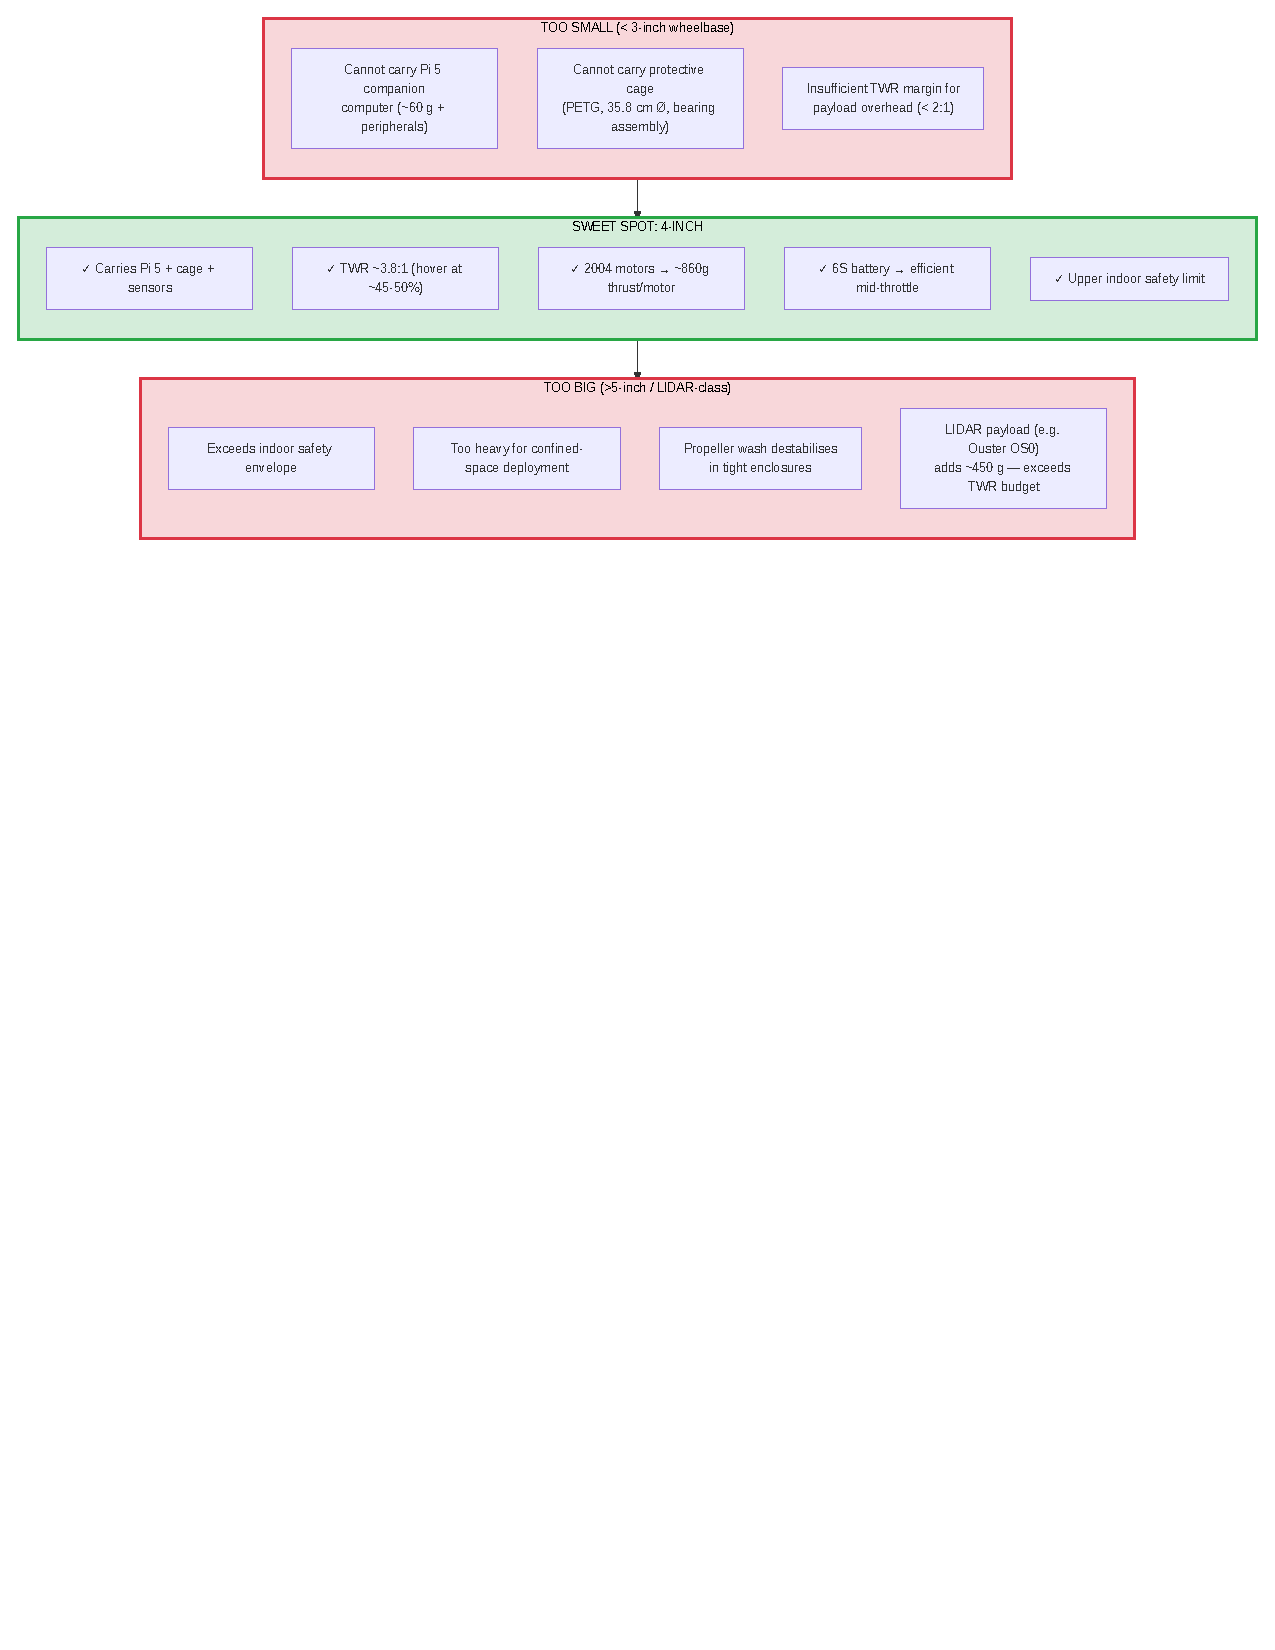
\includegraphics[width=0.95\textwidth]{Figures/drone_sizing_tradeoff.pdf}
    \caption{The three-way sizing constraint that defines the 4-inch platform: going smaller loses payload capacity; going larger violates indoor safety limits. The 4-inch wheelbase is the upper limit for confined indoor flight while providing sufficient thrust to carry the companion computer and protective cage.}
    \label{fig:drone_sizing_tradeoff}
\end{figure}

\textbf{Lower bound: payload minimum.} The Raspberry~Pi~5 companion computer ($\sim$60\,g plus peripherals) and the PETG (polyethylene terephthalate glycol, a 3D-printing filament) protective cage (35.8\,cm diameter, bearing assembly) together require a minimum thrust budget that class-3-inch and below platforms cannot provide. A typical 3-inch build lacks both the stator diameter and the propeller disc area to lift these components while maintaining a safe TWR (thrust-to-weight ratio) margin.

\textbf{Upper bound: indoor safety ceiling.} The 4-inch propeller class is the practical upper limit for indoor flight in confined spaces.\cite{FindYourPerfect} Larger platforms (5-inch and above) produce propeller wash that destabilises the vehicle in tight enclosures and increase the kinetic energy carried into any collision, raising the barrier to physical survivability. Platforms large enough to carry heavy sensors such as a full-size LIDAR (e.g., Ouster OS0 at $\sim$450\,g) exceed the thrust budget while also exceeding safe indoor operating dimensions.

\textbf{The 4-inch sweet spot.} At this scale, 2004-stator motors paired with 4-inch GF4023 propellers on a 6S battery produce sufficient lift for the companion computer and cage while hovering at 45--50\% throttle---near the efficiency peak. The resulting TWR of $\sim$3.8:1 places the drone in the responsive research-autonomy band, with enough thrust to arrest post-collision drift and recover to the commanded setpoint.

\paragraph{Platform Selection: PX4 and Pixhawk 6C}

To address these objectives holistically, PX4 was selected as the autonomous platform. Two platforms currently dominate the open-source UAV ecosystem: ArduPilot and PX4. PX4 was chosen over ArduPilot for its permissive BSD licensing (which allows proprietary extensions, whereas ArduPilot's GPLv3 requires contributed code to remain open), its modular publish-subscribe architecture (uORB), and its well-developed hardware standards under the Dronecode Foundation~\cite{meierPX4NodebasedMultithreaded2015}. PX4's open-source standard is built on modular architecture using \textbf{uORB (microObject Request Broker)}---a publish-subscribe middleware layer suited for plug-and-play development. These factors promised faster integration with the ROS~2 middleware layer and reduced hardware-software troubleshooting. This modularity enables rapid research iteration: novel autonomous behaviors can be implemented as independent modules without modifying the core flight stack.

The \textbf{Pixhawk 6C flight controller} was chosen as the hardware instantiation of the PX4 standard. Critically, Pixhawk is not a monolithic design but represents standardized connector specifications, sensor integration points, and reference schematics managed by the Dronecode Foundation~\cite{simpsonLatestPixhawkOpen2023}. This standardization means:

\begin{itemize}
    \item \textbf{Hardware swappability}: Sensors and peripheral electronics can be upgraded or replaced with components from different manufacturers (Holybro, ARK Electronics, CUAV) without redesigning integration.
    
    \item \textbf{Ecosystem maturity}: Over 1 million Pixhawk-based devices are deployed across commercial, research, and hobbyist applications.\cite{simpsonLatestPixhawkOpen2023}
    
    \item \textbf{Sensor integration}: The Pixhawk 6C includes integrated IMU and compass. Specifically, it features redundant inertial measurement units with onboard ICM-42688-P and BMI088 accelerometers/gyroscopes, plus an IST8310 magnetometer, with temperature-controlled operation via onboard heating resistors.\cite{TechnicalSpecificationHolybro2025, PX4Docs, Pixhawk6C6C} This eliminates the need for custom sensor fusion code---allowing focus on the research question rather than flight control tuning.
\end{itemize}

The 6C's form factor (84.8 \(\times\) 44 \(\times\) 12.4 mm) justifies the 4-inch drone design choice.\cite{TechnicalSpecificationHolybro2025} Four-inch platforms represent the upper practical limit for indoor flight while remaining large enough to carry meaningful payloads.

\paragraph{Thrust-to-Weight and Efficiency Rationale}

The design targets a \textbf{thrust-to-weight ratio (TWR) of approximately 3.8:1}, positioning the platform in the research/autonomous zone where hover occurs at roughly 45--50\% throttle. This mid-throttle hover is deliberate: motor efficiency peaks at 40--70\% throttle, and hovering at 50\% reserves substantial headroom for autonomous obstacle avoidance, gust rejection, and post-collision recovery. Hovering at or near 100\% throttle leaves zero control margin.\cite{oscarHowChooseFPV2024}

\paragraph{Motor and Battery Selection}

\textbf{EMAX ECOII 2004 1600KV} motors were selected. The 2004 stator (20\,mm diameter, 4\,mm height) provides high torque at mid-throttle while the low 1600\,KV rating (1600\,RPM per volt) is matched to a \textbf{6S LiPo battery} (22.2\,V nominal). On this voltage, the motors deliver approximately 860\,g static thrust each under 4-inch GF4023 propellers---a combined 3,440\,g.\cite{drone24hoursTMotorF20041700KV, oscarHowChooseFPV2024} The 6S voltage also places the practical RPM ($\sim$24,000--28,000 under load) within the 4-inch propeller's efficient range, avoiding excessive tip speeds.

\paragraph{Efficiency Advantage of 6S over 4S}

The choice of a 6-cell battery over a 4-cell alternative is driven by efficiency. At a given thrust level, higher voltage draws proportionally lower current, reducing resistive ($I^2R$) losses in the battery, ESCs, and motor windings. Empirically, 6S systems exhibit superior efficiency up to approximately 45\% throttle.\cite{recursionlabsRecursionLabs6s2021}

\textbf{Voltage sag}---the temporary voltage drop under high-current discharge, caused by battery internal resistance ($V_{\text{drop}} = I \times R_{\text{internal}}$)---is proportionally less severe at higher baseline voltages. Under an equivalent current spike, a 4S pack may sag by over 30\% of its nominal voltage, whereas an equivalent-quality 6S pack sees a smaller relative drop.\cite{oscarUsingLiPoBatteries2025} For autonomous flight, where the controller expects a predictable motor response, excessive sag introduces a latency between commanded and actual thrust that degrades control stability during rapid maneuvers. Higher baseline voltage provides a larger operating margin against this effect. The detailed derivation is given in the \hyperref[sec:annex_hardware]{Annex}.

\subsection{System Architecture}

The autonomous flight stack is organised into five layers, illustrated in \autoref{fig:architecture}: Hardware \& Firmware, Middleware, ROS~2 Environment, High-Level Control, and Data \& Analysis. Each layer was selected or developed to address the specific constraints of collision-resilient flight in signal-denied, confined spaces. An external Motion Capture subsystem and a standalone User Input node complete the architecture outside the layered stack.

\begin{landscape}
\begin{figure}[htbp]
    \centering
    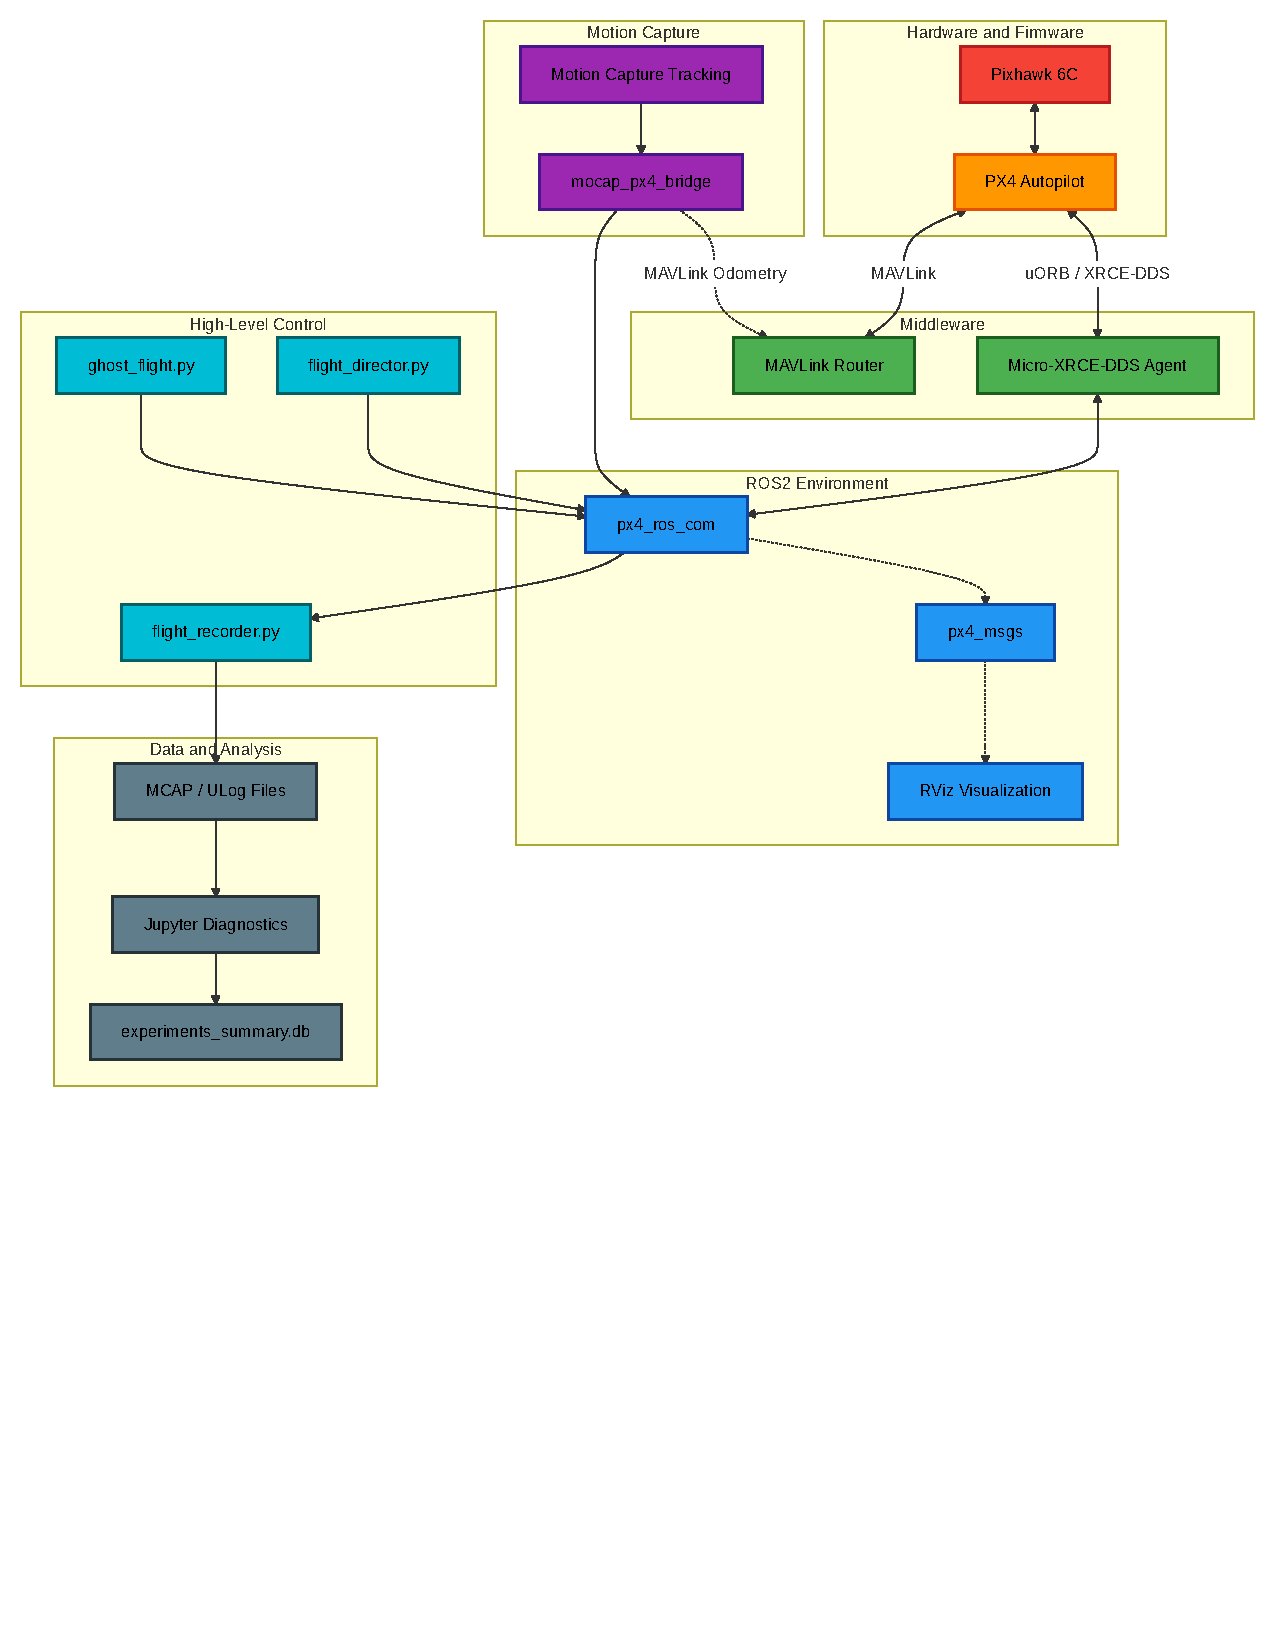
\includegraphics[width=1.45\textwidth]{Figures/architecture.pdf}
    \caption{Drone software stack architecture: PX4 flight controller (red), uXRCE-DDS middleware (green), ROS~2 environment (blue) with \texttt{px4\_msgs} flowing into \texttt{px4\_ros\_com}, high-level control nodes (teal) including the \texttt{flight\_director.py} state machine driven by Mission and User Input, and the data pipeline (grey) routing MCAP/ULog files through DB Pipeline to Experiment Summary and Jupyter Diagnostics. Motion capture (purple) enters via a Wi-Fi multicast link.}
    \label{fig:architecture}
\end{figure}
\end{landscape}

\subsubsection{Hardware Platform}

The companion computer is a \textbf{Raspberry Pi 5} running Ubuntu 24.04. It handles all high-level autonomy: waypoint navigation, MoCap data ingestion, offboard control logic, and telemetry logging. The Pi 5 communicates with the flight controller over UART (TELEM2) and mounts directly above it within the 4-inch frame envelope.

\subsubsection{Flight Controller}

The \textbf{Pixhawk 6C} runs PX4 Autopilot firmware (\texttt{v1.16.1rc}) and is responsible for low-level attitude control, motor mixing, and sensor fusion. Its dual IMU redundancy (ICM-42688-P and BMI088) and onboard IST8310 magnetometer are fused in the EKF2 estimator alongside external vision odometry from the MoCap system. The magnetometer is disabled for indoor operation to prevent interference with MoCap yaw data. The full parameter configuration is given in the repository \texttt{README.md}.

\subsubsection{Motion Capture Integration}

External state estimation is provided by an \textbf{OptiTrack Prime\textsuperscript{x}} 13-camera system streaming at 120\,Hz via NatNet. The \texttt{motion\_capture\_tracking} ROS 2 node receives the multicast stream, and the \texttt{mocap\_px4\_bridge} node transforms the poses from the MoCap ENU frame to PX4's NED/FRD convention, publishing them to \texttt{/fmu/in/vehicle\_visual\_odometry}. The EKF2 estimator fuses this external vision with the onboard 250\,Hz IMU data, bridging any MoCap tracking dropouts through inertial propagation.

\subsubsection{Communication Middleware}

The flight controller and companion computer communicate over a UART serial link (TELEM2, 921\,600 baud). During experimental flights, the link uses \textbf{uXRCE-DDS} exclusively: the PX4 uXRCE-DDS client publishes internal uORB topics (\texttt{vehicle\_odometry}, \texttt{vehicle\_status}, \texttt{actuator\_motors}) to the ROS 2 node graph via \texttt{MicroXRCEAgent} running on the Pi 5. A secondary \textbf{MAVLink} stream can be enabled on the same port for ground-station debugging (QGroundControl), but the two protocols are not used simultaneously during active data collection.

\subsubsection{Software Framework}

\paragraph{Source Submodules}

The ROS~2 workspace integrates several external repositories as Git submodules, providing the interface layer between the high-level autonomy code and the low-level PX4 flight stack:

\begin{lstlisting}[basicstyle=\ttfamily\footnotesize,numbers=none,caption={Source submodules under \texttt{src/} providing the ROS~2--PX4 interface layer.},label={lst:submodules}]
src/
  px4_msgs/                    # PX4 message definitions (uORB <-> ROS 2)
  px4_ros_com/                 # Frame transforms & utility libraries
  Micro-XRCE-DDS-Agent/        # uXRCE-DDS middleware bridge agent
  motion_capture_tracking/     # OptiTrack NatNet receiver node
  mocap_px4_bridge/            # ENU -> NED coordinate transformer
  PX4-Autopilot/               # PX4 firmware source (SITL builds only)
\end{lstlisting}

Three of these are critical for the MoCap-to-PX4 chain: \texttt{px4\_msgs} provides the interface message definitions (ROS~2 \texttt{.msg} files mirroring PX4 uORB topics), \texttt{px4\_ros\_com} handles frame transformations (ENU to NED/FRD), and \texttt{mocap\_px4\_bridge} publishes the transformed poses to \texttt{/fmu/in/vehicle\_visual\_odometry}.

\paragraph{The Flight Director}

The \texttt{flight\_director.py} node was developed directly from the PX4 ROS~Com offboard control examples, inheriting their structure for heartbeat publishing, offboard mode switching, and trajectory setpoint generation. It serves as the primary mission executor:

\begin{itemize}
    \item \textbf{State machine}: Implements the waypoint state machine shown in \autoref{fig:waypoint_state_machine}, transitioning through DISARMED $\to$ TAKEOFF (WP0) $\to$ WP\_stage (U-turn) $\to$ Exp.\ Start-point (WP1) $\to$ Exp.\ End-point (WP2) $\to$ Recovery (WP3) $\to$ (auto-loop to WP\_stage, or LANDING). Each state transition publishes a waypoint-identifier message that drives the event segmenter.
    \item \textbf{Offboard control}: Publishes \texttt{TrajectorySetpoint} messages to \texttt{/fmu/in/trajectory\_setpoint} with explicit velocity feedforward (\texttt{hb.velocity = True}). Subscribes to \texttt{/fmu/out/vehicle\_status} for telemetry feedback.
    \item \textbf{Safety enforcement}: Monitors the geofence boundary with the cage-radius offset (17.9\,cm) subtracted, and triggers an emergency landing on breach, MoCap loss, or spacebar kill-switch.
\end{itemize}

The complete experimental pipeline, from hardware through the ROS~2 node graph to telemetry storage, is illustrated in \autoref{fig:experiments_pipeline}.

\begin{figure}[htbp]
    \centering
    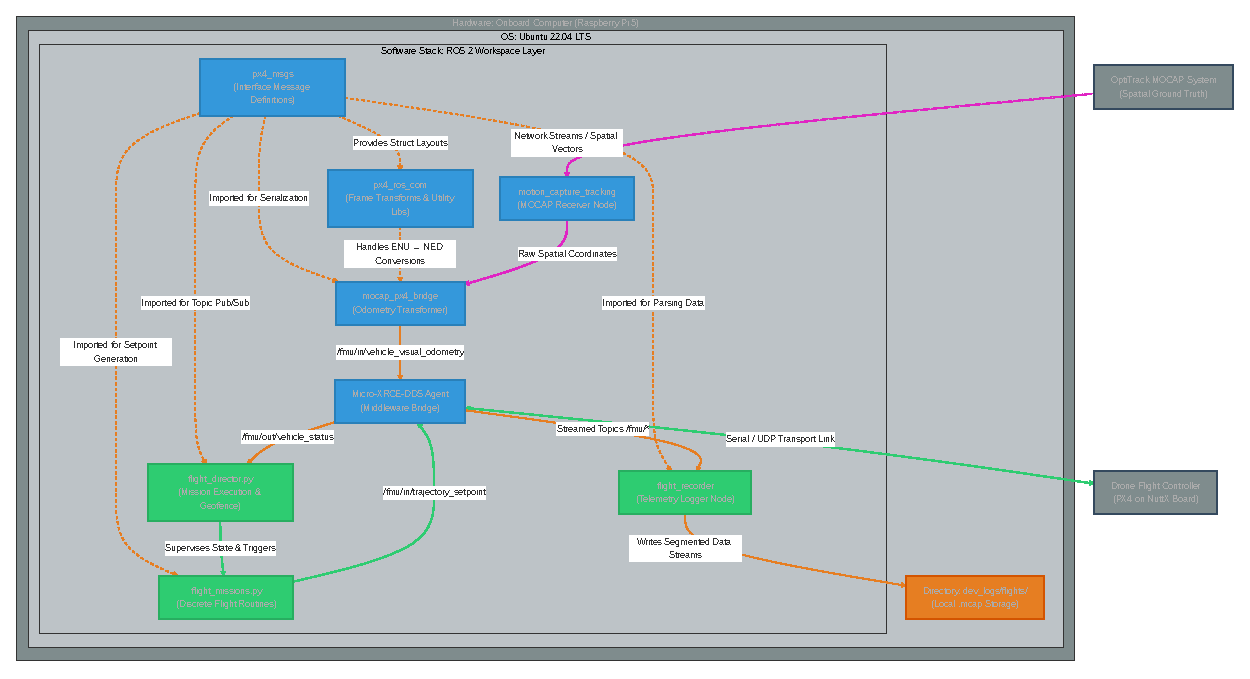
\includegraphics[width=\textwidth]{Figures/experiments_pipeline.pdf}
    \caption{Experiment pipeline showing hardware components, ROS~2 software stack, data flow from MOCAP through the agent to PX4, and telemetry logging to MCAP storage.}
    \label{fig:experiments_pipeline}
\end{figure}

The \texttt{flight\_missions.py} module provides discrete flight routines (column sweep, hover verification), while \texttt{flight\_recorder.py} logs synchronised topic data to segmented \texttt{.mcap} files, one per loop iteration.



\subsubsection{Frame and Cage Design}

The protective cage design draws on two established geometries from the collision-resilience literature. Mahmud et al.\cite{mahmudDevelopmentCollisionResilient2021} compared a freely rotating gimbal sphere against a G\"omb\"oc-shaped shell (a mono-monostatic body with a single stable equilibrium), concluding the turtle-like G\"omb\"oc form was superior for self-righting after impacts. The cage adopted for this work shares the rotating-shell principle: a PETG-printed spherical cage of 35.8\,cm diameter, mounted on a bearing assembly that allows the outer shell to spin freely upon contact with an obstacle. This mechanical decoupling converts linear collision momentum into rotational energy, shunting impact shock away from the central fuselage and flight controller.

The fixed-cage control configuration uses identical geometry but rigidly mounts the outer shell to the frame, eliminating the bearing's rotational degree of freedom. All other parameters (mass, diameter, material, propeller clearance) are held constant between the two configurations, isolating the effect of the bearing mechanism as the single experimental independent variable.

\
\clearpage
\section{Experiments and Results}

The Results chapter presents a deliberately structured progression from raw mechanical measurements to inferential analysis. Each plot represents a deliberate analytical choice: the figures are ordered to first establish the baseline dataset and spatial context, then characterise the physical dynamics of impact (deceleration, vibration, trajectory deviation), and finally assess whether the onboard IMU signatures alone can recover the impact angle without external MoCap ground truth. Comparative metrics between the Fixed Cage and Rotating Cage configurations are presented side-by-side throughout, enabling direct visual and statistical comparison of the bearing mechanism's effect.

To evaluate the operational and protective capabilities of the drone cage and to assess what indication of impact angle might be recoverable from onboard sensors, physical collision tests were conducted. This section details the experimental setup, the software pipeline used to capture the data, and the direct mechanical results, comparing the performance of the fixed cage against the freely rotating cage.

\subsection{Motion Capture Setup}

External state estimation is provided by a \textbf{6-camera OptiTrack Prime~22} system streaming at 120\,Hz via the Motive software platform (Mudfish network middleware). The Prime~22 offers sub-millimetre positional accuracy at short range, sufficient for the $\sim$5\,m$\times$5\,m capture volume used in these experiments.

The \texttt{motion\_capture\_tracking} ROS~2 node receives the multicast stream from Motive, and the \texttt{mocap\_px4\_bridge} node transforms the poses between coordinate frames before publishing them to \texttt{/fmu/in/vehicle\_visual\_odometry}.

\paragraph{Coordinate Frame Transformations}

Coordinate frame conventions differ between MoCap and PX4. ENU is a ground-fixed frame where the $X$~axis points East, $Y$~points North, and $Z$~points Up; the vehicle body frame has $X$~toward the front, $Z$~up, and $Y$~toward the left. PX4's internal state estimator operates in the \textbf{NED (North-East-Down)} frame, where $X$~points North, $Y$~points East, and $Z$~points Down; the corresponding vehicle body frame (\textbf{FRD}, Forward-Right-Down) has $X$~toward the front, $Z$~down, and $Y$~accordingly. \autoref{fig:coordinate_frames} shows both conventions side by side.\footnote{Software documentation available at: \url{https://docs.px4.io/main/en/tutorials/motion-capture}}

\begin{figure}[htbp]
    \centering
    \includegraphics[width=0.85\textwidth]{Figures/coordinate_frames_NEDvsENU.png}
    \caption{NED (left) and ENU (right) coordinate frame conventions. Adapted from PX4 documentation~\footnote{Software documentation available at: \url{https://docs.px4.io/main/en/tutorials/motion-capture}}.}
    \label{fig:coordinate_frames}
\end{figure}

The \texttt{mocap\_px4\_bridge} performs this transform in two steps: first, a static rotation maps ENU to NED ($X_{\text{NED}} = Y_{\text{ENU}}$, $Y_{\text{NED}} = X_{\text{ENU}}$, $Z_{\text{NED}} = -Z_{\text{ENU}}$); second, the NED pose is rotated into the FRD body frame using the vehicle's current attitude quaternion. The resulting \texttt{VehicleVisualOdometry} message is published at 120\,Hz to \texttt{/fmu/in/vehicle\_visual\_odometry}.

The EKF2 estimator fuses this external vision with the onboard 250\,Hz IMU data. During steady, unoccluded flight, this fusion produces velocity estimates that align closely with the MoCap-derived ground truth, as shown in Figure~\ref{fig:ekf_validation} for representative flights from both cage configurations.

\paragraph{EKF Validation Under MoCap Occlusion}

During the exact millisecond of physical impact, the protective cage and column structure physically block the infrared camera's line-of-sight to the drone's reflective markers. This transient marker occlusion causes the MoCap tracking data to glitch. When velocity and acceleration are derived from position by numerical differentiation, even a single-frame position glitch produces a massive, non-physical spike in the resulting kinematic profile. The Savitzky-Golay differentiation filter cannot remove this artefact---it amplifies any discontinuity in the underlying data. Figure~\ref{fig:mocap_dropout} illustrates this failure: the MoCap-derived velocity and acceleration traces exhibit violent, unphysical excursions at the impact instant ($t = 0$), while the EKF2 odometry remains smooth and continuous throughout the event.

The EKF2 does not rely solely on the external vision stream. It continuously fuses the onboard 250\,Hz IMU accelerometer and gyroscope data into its state estimate. When the MoCap feed momentarily degrades, the inertial propagation bridges the gap without introducing noticeable drift. The smooth, physically plausible EKF velocity profile through the collision window---visible in Figure~\ref{fig:mocap_dropout}---confirms that the filter successfully compensates for the optical dropout.

\begin{figure}[htbp]
    \centering
    \includegraphics[width=0.95\textwidth]{plots/Fixed Cage Kinetic Profile (Raw).png}
    \caption{Figure A: MoCap dropout during impact. The Savitzky-Golay filtered MoCap velocity (blue, top panel) and acceleration (green, bottom panel) exhibit severe non-physical spikes at $t = 0$, caused by marker occlusion at the instant of column contact. The EKF2 odometry (red) remains smooth and continuous, bridging the dropout via inertial propagation.}
    \label{fig:mocap_dropout}
\end{figure}

\begin{figure}[htbp]
    \centering
    \includegraphics[width=0.95\textwidth]{plots/EKF Dual Comparison Fixed vs Rotating.png}
    \caption{Figure B: EKF vs.\ MoCap velocity validation during clean, unoccluded flight for representative Fixed Cage (left) and Rotating Cage (right) flights. The close alignment between the two traces confirms that the EKF2 accurately mirrors the MoCap ground truth under normal tracking conditions.}
    \label{fig:ekf_validation}
\end{figure}

Based on this validated alignment, EKF odometry is used as the primary source of velocity and acceleration data for all kinematic calculations through the collision window. The raw MoCap position data is retained solely for geometric reference (impact angle computation, clearance measurement, and trajectory visualization)---calculations that do not require numerical differentiation and are therefore insensitive to transient position glitches.

\begin{figure}[htbp]
    \centering
    \includegraphics[width=0.85\textwidth]{plots/Impact Angle Distribution by Cage Configuration.png}
    \caption{Distribution of measured impact angles for both cage configurations. The rotating cage sample is shifted toward the lower end of the $45^\circ$ approach condition (mean~$\pm$~SD: $40.6 \pm 11.5^\circ$) compared to the fixed cage ($46.7 \pm 13.0^\circ$), reflecting variance in collision geometry across passes.}
    \label{fig:impact_angle_distribution}
\end{figure}

\subsection{Experimental Setup}
\subsubsection{Experiment Environment and Collision Target}
The physical experiments were conducted at the REALLAB at the IT University of Copenhagen (ITU) within an OptiTrack Motion Capture (MoCap) environment. A vertically oriented cylindrical cardboard column, internally reinforced with an aluminum profile, was anchored to the floor and ceiling to serve as the static collision target. The column oscillates slightly when subjected to manual force, but no additional structural supports were added in order to prevent any occlusion of the MoCap cameras, preserving their function as the primary reference point for the drone's spatial positioning. Analysis of the MoCap data confirmed that obstacle displacement during impacts was below the system's millimetre tracking resolution. Therefore, energy absorption by the environment is considered negligible.

\subsubsection{Experiment Control and Data Collection}
The experimental platform relies on an integrated software architecture designed to bridge abstracted trajectory generation with real-time hardware constraints. The low-level flight stack utilizes PX4 Autopilot firmware on a NuttX real-time operating system (RTOS), with internal state estimation handled strictly by an Extended Kalman Filter (EKF2).\footnote{Software documentation available at: \url{https://docs.px4.io/main/en/flight_controller/pixhawk6c}} \textbf{L1 Node} --- the EKF2 is the primary source of velocity state data for the entire analysis pipeline, fused from the onboard IMU data logged at 250\,Hz (the rate at which the EKF2 pipeline ingests the raw accelerometer and gyroscope data) and the 120\,Hz external MoCap vision odometry stream.

High-level position commanding is managed within a ROS~2 abstraction layer running on an external offboard computing node. Real-time topic translation between the ROS~2 node graph and the internal PX4 uORB messaging system is handled via a micro-XRCE-DDS agent.

To orchestrate the experimental runs, a custom software component named \texttt{flight\_director.py} was developed. This script functions as an automated mission execution environment, systematically enforcing geofence safety parameters. The flight director automates the data collection pipeline by initializing synchronized telemetry recordings, saving each distinct flight loop into an independent \texttt{.mcap} file. These files were subsequently parsed using a custom Python database pipeline to calculate the physical variables presented in the following results.

The complete experimental pipeline, from hardware components through the ROS~2 software stack and MoCap integration to telemetry storage, is illustrated in \autoref{fig:experiments_pipeline}.

\subsubsection{Data Processing for Collision Analysis}
\label{sec:mocap_ekf2}

During the exact millisecond of physical impact, the protective cage structures transiently occlude the drone's reflective markers. This occlusion frequently caused the MoCap tracking publish rate to drop below the critical 30\,Hz failsafe threshold, occasionally plummeting to $\sim$10\,Hz. When relying purely on raw spatial differentiation, these temporal gaps produced massive, artificial high-frequency spikes in the calculated kinematic profiles, even when applying Savitzky-Golay filtering.

To resolve this without sacrificing data fidelity, the analysis pipeline bypasses raw spatial differentiation for velocity and acceleration entirely. Instead, velocity states are extracted directly from the internal PX4 Extended Kalman Filter (\texttt{vehicle\_odometry.velocity}). Because the EKF2 continuously fuses the onboard 250\,Hz IMU data, it bridges external vision dropouts using inertial propagation, providing a smooth and physically truthful velocity profile throughout the collision event.

\subsubsection{Pre-Computed Path and Waypoint Configuration}

To reiterate, this physical collision framework represents the actual experimental flight tests conducted, from which all the data in this thesis stems. The system uses a pre-computed ROS~2 waypoint trajectory to ensure every pass is mechanically identical. The exact spatial path, including the approach, impact, and recovery segments, is detailed in Figure~\ref{fig:mission_geometry}.

\begin{figure}[h!]
    \centering
    \includegraphics[width=\textwidth]{plots/45° Column Collision Loop Full Mission Geometry.png}
    \caption{Full mission geometry for the $45^\circ$ collision experiment. The dotted red line traces the closed-loop waypoint path. Waypoints correspond to the state machine: \texttt{WP\_stage} initiates the forward approach; Exp.\ Start-point (\texttt{WP1}) marks the start of the high-momentum sweep leg; Exp.\ End-point (\texttt{WP2}) marks the exit; and Recovery (\texttt{WP3}) is the hold position. \textit{An additional \texttt{WP0} (Takeoff) exists off-diagram at the drone's physical starting location on the floor, utilized only once at the start of the flight. The column obstacle is shown at the centre. Note that the `ideal' line between Exp.\ Start-point (\texttt{WP1}) and Exp.\ End-point (\texttt{WP2}) dictates the trajectory, and Exp.\ End-point (\texttt{WP2}) possesses a 15~cm diameter acceptance leeway to register the waypoint as reached.}}
    \label{fig:mission_geometry}
\end{figure}

% ======================================================================
\subsection{Experimental Kinematics and Spatial Recovery}
\label{sec:deviation_from_norm}
% ======================================================================

This section reports the macro-spatial kinematics of the collisions. As detailed in Table~\ref{tab:dataset_baseline}, the analysis is based on 179 executed passes, yielding 168 recorded passes and 127 verified impacts across both configurations.

\begin{table}[h!]
\centering
\caption{Dataset baseline: total flight passes, verified structural impacts, and the isolation criteria used to distinguish genuine collisions from near-miss transits.}
\label{tab:dataset_baseline}
\resizebox{\textwidth}{!}{%
\begin{tabular}{lcc}
\toprule
\textbf{} & \textbf{Count} & \textbf{Notes} \\
\midrule
Total flight passes executed & 179 & Across all experimental sessions \\
\addlinespace
Verified structural impacts & 127 & Confirmed via telemetry inspection + cage-radius verification \\
\addlinespace
\hspace{0.5em}-- Fixed Cage & 67 & \\
\hspace{0.5em}-- Rotating Cage & 60 & \\
\addlinespace
Isolation criterion & -- & Physical contact confirmed when $d_{\text{centre}} < r_{\text{column}} + r_{\text{cage}} = 0.224$~m \\
\addlinespace
Battery drain rate (\%\,min$^{-1}$) & 21.3 & Both configurations; full unsliced flight sessions \\
\bottomrule
\end{tabular}}%
\end{table}

\subsubsection{Trajectory Visualisation and Mission Outcomes}
\label{sec:horizontal_kinematics}

To evaluate the drone's horizontal flight dynamics, this analysis focuses on the spatial divergence between the pre-computed commanded path and the actual trajectory executed. Visualizing this path deviation in Figure~\ref{fig:horizontal_kinematics} displays the physical trajectories executed during the impacts. A breakdown of the specific mission outcomes (impacts vs.\ no impacts across angles) is provided in Table~\ref{tab:mission_outcomes}.

\begin{figure}[h!]
    \centering
    \includegraphics[width=\textwidth]{plots/Experiment 2D horizontal visualization.png}
    \caption{2D horizontal visualization of the experiment flight paths. The plot compares commanded versus executed trajectories for both fixed and rotating cage configurations across the collision sweep leg, showing spatial deviation, impact coordinates, and recovery overshoot required to stabilize lateral drift.}
    \label{fig:horizontal_kinematics}
\end{figure}

\begin{table}[h!]
    \centering
    % Auto-generated by plot_mission_outcome_table()
% Requires: \usepackage{booktabs}
\begin{tabular}{lrrrrrrr}
\toprule
 & \rotatebox{90}{\textsf{N}} & \rotatebox{90}{\textsf{No Impact}} & \rotatebox{90}{\textsf{{<\,}30°}} & \rotatebox{90}{\textsf{30–40°}} & \rotatebox{90}{\textsf{40–50°}} & \rotatebox{90}{\textsf{50–60°}} & \rotatebox{90}{\textsf{60–90°}} \\
\midrule
\multicolumn{8}{l}{\textbf{Rotating Cage}} \\
\midrule
\quad 45° & 50 & 2 & 9 & 21 & 13 & 5 & 0 \\
\quad 75° & 31 & 19 & 0 & 2 & 2 & 3 & 5 \\
\quad \textbf{All} & 81 & 21 & 9 & 23 & 15 & 8 & 5 \\
\addlinespace
\multicolumn{8}{l}{\textbf{Fixed Cage}} \\
\midrule
\quad 45° & 56 & 5 & 3 & 18 & 13 & 10 & 7 \\
\quad 75° & 31 & 15 & 2 & 0 & 4 & 5 & 5 \\
\quad \textbf{All} & 87 & 20 & 5 & 18 & 17 & 15 & 12 \\
\bottomrule
\end{tabular}
%% Data: experiments_summary.db → flights_summary (81× Rotating, 87× Fixed flights)

    \caption{Mission outcome summary across all 168 recorded passes. Flights are categorised by cage configuration, target approach angle ($45^\circ$ and $75^\circ$), and the measured impact angle at the collision instant. The ``No Impact'' column counts passes where the drone cleared the column without physical contact.}
    \label{tab:mission_outcomes}
\end{table}

\subsubsection{Spatial Trajectory and Recovery Metrics}
\label{sec:clearance_sdld}

The spatial consequences of the physical impacts are quantified by assessing the clearance, the worst-case deviation, and the total recovery area. These values are summarized in Table~\ref{tab:spatial_metrics}.

\textbf{Obstacle clearance} represents the closest physical approach. The rotating cage exhibits a larger mean negative clearance, meaning it incurs deeper into the column boundary (Rotating: $\mu = -0.637 \pm 0.172$~m; Fixed: $\mu = -0.470 \pm 0.165$~m).

\textbf{Maximum Trajectory Deviation} ($d_{\text{max}}$) is the peak perpendicular distance between the executed MoCap track and the commanded `ideal' reference line. This ideal line is drawn exactly from the coordinate where the drone was commanded forward (\texttt{WP1}) to the exact target coordinate it must reach (\texttt{WP2}, which includes a 15~cm precision leeway). This metric captures the single worst-case excursion during the obstacle transit. According to Table~\ref{tab:spatial_metrics}, the rotating cage recorded a maximum trajectory deviation of $131.0 \pm 32.1$~mm, while the fixed cage recorded $118.4 \pm 30.4$~mm.

\textbf{Spatial Integral of Absolute Error} (SIAE) measures the total spatial area footprint of the recovery phase. Table~\ref{tab:spatial_metrics} shows the spatial area of the recovery phase was $120.4 \pm 32.2 \times 10^{-3}~\text{m}^2$ for the rotating cage and $117.4 \pm 33.2 \times 10^{-3}~\text{m}^2$ for the fixed cage.

Finally, the \textbf{Path Spread (RMSLD)} quantifies how tightly the drone tracks the ideal line over the entirety of the obstacle passage. To visualize this overall consistency across all flight tests, the overlaid paths of all flights are shown in Figure~\ref{fig:path_heatmap}. As extracted from the dataset, the path spread is recorded at $40.3 \pm 9.8$~mm for the rotating cage and $37.4 \pm 11.0$~mm for the fixed cage.

\begin{figure}[htbp]
    \centering
    \includegraphics[width=\textwidth]{plot_16_path_heatmap.png}
    \caption{Path overlay of all impact flights for both cage configurations. Each flight trajectory is plotted at low opacity, showing the aggregate spatial footprint of the collision sweep for Rotating Cage (left, blue) and Fixed Cage (right, red). The dashed line marks the nominal commanded path.}
    \label{fig:path_heatmap}
\end{figure}

Based on the data reported above, the spatial recovery metrics suggest that the rotating cage's bearing mechanism does not expand the final recovery footprint required by the standard flight controller settings. This pattern is further evaluated by comparing the worst-case excursions and recovery consistency across configurations.

The two complementary metrics---maximum deviation and SIAE---confirm that a brief large excursion and a prolonged small offset can produce similar SIAE values. The rotating cage exhibited a slightly wider maximum trajectory deviation than the fixed cage. A Mann-Whitney U test confirms this difference is statistically significant ($U = 2484$, $p = 0.022$), though the effect size is small (Cohen's $d = 0.41$). However, the total spatial area required by the PID controller to arrest the drift and return to the setpoint (SIAE) remains nearly identical between both configurations ($U = 2009$, $p = 0.998$, not significant).

\begin{table}[htbp]
\centering
\caption{Spatial and Clearance Metrics. Summary of key comparative spatial metrics between cage configurations. All values are mean~$\pm$~standard deviation.}
\label{tab:spatial_metrics}
\resizebox{\textwidth}{!}{%
\begin{tabular}{lccc}
\toprule
\textbf{Metric} & \textbf{Rotating Cage} & \textbf{Fixed Cage} & \textbf{Statistical Test} \\
\midrule
Obstacle Clearance (m) & $-0.637 \pm 0.172$ & $-0.470 \pm 0.165$ & --- \\
\addlinespace
Max. Trajectory Deviation (mm) & $131.0 \pm 32.1$ & $118.4 \pm 30.4$ & $U=2484$, $p=0.022$, $d=0.41$ \\
\addlinespace
SIAE Recovery Area (\texttimes 10$^{-3}$\,m$^{2}$) & $120.4 \pm 32.2$ & $117.4 \pm 33.2$ & $U=2009$, $p=0.998$\,(n.s.) \\
\addlinespace
Path Spread RMSLD (mm) & $40.3 \pm 9.8$ & $37.4 \pm 11.0$ & --- \\
\bottomrule
\end{tabular}}%
\end{table}

% ======================================================================
\subsection{Impact Acceleration and Vibrations}
\label{sec:impact_acceleration_vibrations}
% ======================================================================

To understand the physical forces at contact, we evaluate the IMU acceleration and gyroscopic data. During these extreme stress tests---consisting of repeated, high-throttle crash recoveries---the platform averaged a heavy continuous battery drain of 21.3\% per minute. Because such voltage drops can affect motor authority, it was necessary to confirm that battery depletion did not secretly skew the deceleration data. The covariance with the starting battery percentage is summarised in Table~\ref{tab:deceleration_battery}.\label{sec:efficiency_baseline}

\begin{table}[h!]
\centering
\caption{Impact Deceleration and Battery Covariance. Summary of impact deceleration and its covariance with starting battery percentage. The near-zero Huber slopes confirm that battery state-of-charge did not confound the deceleration measurements. Note: The relative difference can be expressed either as a 37.2\% reduction from the fixed baseline, or equivalently, the fixed cage experiencing a 59\% higher deceleration than the rotating cage.}
\label{tab:deceleration_battery}
\begin{tabular}{lcc}
\toprule
\textbf{Metric} & \textbf{Fixed Cage} & \textbf{Rotating Cage} \\
\midrule
Mean Max.\ Deceleration ($\text{m/s}^2$) & $-1.64 \pm 0.64$ & $-1.03 \pm 0.50$ \\
Relative Difference & Baseline & $-37.2\%$ reduction \\
Battery Covariance (Huber Slope) & $-0.005$ & $0.000$ \\
\bottomrule
\end{tabular}
\end{table}

As detailed in Table~\ref{tab:deceleration_battery}, the rotating cage recorded a mean maximum deceleration of $-1.03 \pm 0.50$~m/s$^2$, while the fixed cage recorded $-1.64 \pm 0.64$~m/s$^2$. To clarify the relative performance differences, these values are expressed as absolute magnitudes (representing the raw physical force transferred to the airframe).

When evaluating how much the fixed cage amplifies the impact forces relative to the rotating cage, the rotating cage serves as the baseline ($D_{\text{rot}} = 1.03$):
\[ \text{Relative Increase} = \frac{|D_{\text{fix}}| - |D_{\text{rot}}|}{|D_{\text{rot}}|} = \frac{1.64 - 1.03}{1.03} \approx 0.592 \]
This demonstrates a 59.2\% higher maximum deceleration for the fixed cage.

Conversely, when evaluating the mitigating effect of the bearing mechanism, the standard fixed cage serves as the baseline ($D_{\text{fix}} = 1.64$):
\[ \text{Relative Reduction} = \frac{|D_{\text{fix}}| - |D_{\text{rot}}|}{|D_{\text{fix}}|} = \frac{1.64 - 1.03}{1.64} \approx 0.372 \]
This demonstrates a 37.2\% reduction in impact deceleration achieved by the rotating cage.

An independent samples t-test (Welch) confirms this difference is statistically significant ($t(124.7) = 6.00$, $p < 0.001$, Cohen's $d = 1.05$). This strong statistical significance points to a regular, normalized data distribution, confirming the high reliability and relevancy of the obtained deceleration values.

\paragraph{IMU Time-Series: Individual and Aggregated Signatures}

Figure~\ref{fig:imu_dynamics_pair} presents the acceleration and gyroscopic traces. The upper panel shows representative single-flight traces. The lower panel aggregates all 127 flights. In the aggregated data, the overlaid individual traces reveal a visually narrower spread of linear acceleration peaks for the rotating cage, alongside a shorter median gyroscopic peak duration compared to the fixed cage.

\begin{figure}[htbp]
    \centering
    \begin{subfigure}{\textwidth}
        \centering
        \includegraphics[width=\textwidth]{plots/Combined IMU Collision Dynamics.png}
        \caption{Representative single-flight traces for Rotating Cage (left) and Fixed Cage (right).}
        \label{fig:combined_imu_dynamics}
    \end{subfigure}
    \vspace{1em}
    \begin{subfigure}{\textwidth}
        \centering
        \includegraphics[width=\textwidth]{plots/Aggregated IMU Collision Dynamics Across All Flights.png}
        \caption{Aggregate overlay of all 127 flights with median profiles.}
        \label{fig:aggregated_imu_dynamics}
    \end{subfigure}
    \caption{IMU collision dynamics at two granularities: (a) representative individual flights reveal the per-event shock and decay signature; (b) aggregation across all 127 flights confirms the pattern is systematic. Together they establish that the rotating cage consistently attenuates both the magnitude and the variability of impact-induced vibration.}
    \label{fig:imu_dynamics_pair}
\end{figure}

\paragraph{Axis-Resolved IMU Component Analysis}

Disaggregating by axis, Figure~\ref{fig:raw_imu_xyz} shows the X, Y, Z collision window. The Y axis (lateral) records peaks below $\pm 4~\text{m/s}^2$ for the rotating cage, compared to peaks exceeding $\pm 6~\text{m/s}^2$ for the fixed cage.

\begin{figure}[h!]
    \centering
    \includegraphics[width=\textwidth]{plots/Combined IMU XYZ Components.png}
    \caption{Raw acceleration traces for each axis (X, Y, Z) during the collision window. The $Y$~axis (lateral) carries the dominant collision signature in both configurations; the rotating cage reduces peak amplitude by roughly one-third on this channel.}
    \label{fig:raw_imu_xyz}
\end{figure}

The box plots in Figure~\ref{fig:xyz_oscillation_variance} summarise the post-impact stabilisation tail ($t_{\text{impact}} + 0.2\,\text{s}$ to $+3.0\,\text{s}$) across all flights. During steady flight, the rotating cage exhibits a lower variance spread in both the X and Y axes. During impact, the rotating cage records a lower spread in the Y axis, but registers a larger interquartile spread in the Z axis.

\begin{figure}[htbp]
    \centering
    \includegraphics[width=\textwidth]{plots/IMU Vibration Spread by Cage Configuration.png}
    \caption{Box plots of per-axis variance over the post-impact stabilisation tail ($t_{\text{impact}} + 0.2\,\text{s}$ to $+3.0\,\text{s}$). The rotating cage's narrower interquartile ranges confirm that the bearing reduces both peak shock and the duration of residual vibration.}
    \label{fig:xyz_oscillation_variance}
\end{figure}

To provide a holistic view of the drone's subsystem performance, Table~\ref{tab:master_comparison} aggregates the key metrics across kinematics, motor output, attitude control, and vibration. This table highlights several noteworthy differences, specifically that the rotating cage records substantially lower yaw-rate tracking error ($-85\%$) and reduced allocator saturation ($-96\%$) compared to the fixed configuration.

\paragraph{EKF State Estimation Fidelity}

Because the MoCap markers can become occluded during physical contact with the column, it was necessary to verify if the flight controller's internal state estimation could reliably bridge these visual dropouts. Figure~\ref{fig:ekf_validation} plots the EKF-estimated velocity alongside the MoCap-derived velocity over the collision window for representative flights. The two traces track each other closely through the entire collision window. This agreement confirms that the EKF2's inertial propagation reliably bridges the transient MoCap dropout without introducing noticeable drift, justifying the use of EKF telemetry for the collision analysis.

\medskip
The preceding kinematic and vibrational analyses establish that the rotating cage fundamentally alters the physical distribution of collision energy. However, for a drone operating without external motion-tracking, this mechanical advantage is only practically useful if the onboard sensors retain enough information to characterise the impact. As indicated by the IMU feature correlation analysis (see \autoref{fig:imu_correlation}), the relationship between impact angle and inertial response is highly complex and dispersed across multiple axes. This dispersion suggests that simple linear thresholds are insufficient, necessitating a multivariate, non-linear approach to successfully decode the collision geometry from the raw telemetry.

\begin{table}[h!]
\centering
\caption{Comprehensive Performance Summary. Comprehensive comparison of all key performance metrics between cage configurations. Values are mean~$\pm$~standard deviation across all 127 verified impact flights (60 Rotating Cage, 67 Fixed Cage). Arrow direction ($\leftarrow$ or $\rightarrow$) indicates which configuration achieves the favourable outcome for each metric; the $\Delta$ column shows the percentage difference relative to the Fixed Cage baseline.}
\label{tab:master_comparison}
\footnotesize
\setlength{\tabcolsep}{3pt}
\begin{tabular}{lcccr}
\toprule
\textbf{Category / Metric} & \textbf{Rotating} & \textbf{Fixed} & \textbf{$\Delta$ (\%)} & \textbf{Better} \\
\midrule
\multicolumn{5}{l}{\textbf{Kinematics}} \\
~~Peak Decel. Z (m/s$^{2}$) & $10.0\pm4.7$ & $6.57\pm4.00$ & $+52.5$ & $\rightarrow$ Fixed \\
~~Max Traj. Deviation (mm) & $131.0\pm32.1$ & $118.4\pm30.4$ & $+10.7$ & $\rightarrow$ Fixed \\
~~Integ. Rot. Energy (rad) & $0.16\pm0.05$ & $0.24\pm0.07$ & $-33.7$ & $\leftarrow$ Rotating \\
~~Recovery Area (m$^{2}$) & $0.12\pm0.03$ & $0.12\pm0.03$ & $+2.6$ & $\rightarrow$ Fixed \\
~~Path Spread RMSLD (mm) & $40.3\pm9.8$ & $37.4\pm11.0$ & $+7.8$ & $\rightarrow$ Fixed \\
~~Experiment Duration (s) & $7.94\pm1.26$ & $7.88\pm1.76$ & $+0.7$ & $\rightarrow$ Fixed \\
\midrule
\multicolumn{5}{l}{\textbf{Motors \& Energy}} \\
~~Max Actuator Output (\%) & $99.3\pm1.5$ & $99.9\pm0.0$ & $-0.6$ & $\leftarrow$ Rotating \\
\midrule
\multicolumn{5}{l}{\textbf{Attitude Control}} \\
~~Roll Rate RMS (rad/s) & $0.22\pm0.05$ & $0.16\pm0.05$ & $+36.2$ & $\rightarrow$ Fixed \\
~~Pitch Rate RMS (rad/s) & $0.29\pm0.12$ & $0.25\pm0.11$ & $+13.4$ & $\rightarrow$ Fixed \\
~~Yaw Rate RMS (rad/s) & $0.09\pm0.03$ & $0.57\pm0.15$ & $-85.0$ & $\leftarrow$ Rotating \\
\midrule
\multicolumn{5}{l}{\textbf{Control Allocation}} \\
~~Alloc. Sat. Duration (s) & $0.01\pm0.02$ & $0.13\pm0.10$ & $-96.2$ & $\leftarrow$ Rotating \\
~~Max Unalloc. Torque (N\,m) & $0.01\pm0.04$ & $0.01\pm0.02$ & $-2.3$ & $\leftarrow$ Rotating \\
~~Thrust Setpt. Achieved (\%) & $97.3\pm6.9$ & $85.1\pm13.2$ & $+14.4$ & $\leftarrow$ Rotating \\
\midrule
\multicolumn{5}{l}{\textbf{IMU Vibration}} \\
~~Accel X Impact (g) & $0.28\pm0.11$ & $0.29\pm0.13$ & $-3.6$ & $\leftarrow$ Rotating \\
~~Accel Y Impact (g) & $0.26\pm0.08$ & $0.37\pm0.16$ & $-28.6$ & $\leftarrow$ Rotating \\
~~Accel Z Impact (g) & $0.24\pm0.09$ & $0.18\pm0.09$ & $+32.3$ & $\rightarrow$ Fixed \\
~~Accel X Regular (g) & $0.01\pm0.01$ & $0.05\pm0.07$ & $-69.5$ & $\leftarrow$ Rotating \\
~~Accel Y Regular (g) & $0.02\pm0.01$ & $0.10\pm0.11$ & $-77.1$ & $\leftarrow$ Rotating \\
~~Accel Z Regular (g) & $0.05\pm0.01$ & $0.04\pm0.03$ & $+10.8$ & $\rightarrow$ Fixed \\
\midrule
\bottomrule
\end{tabular}
\end{table}

% ======================================================================
\subsection{Intermediate Mechanical Discussion}
\label{sec:intermediate_discussion}
% ======================================================================

Based on the data reported in Sections~\ref{sec:deviation_from_norm} and~\ref{sec:impact_acceleration_vibrations}, several mechanical hypotheses can be formulated regarding the bearing mechanism's effect on collision energy.

First, the trajectory recovery area (SIAE) remained nearly identical between configurations despite a slightly wider initial deviation for the rotating cage. This indicates that the spatial cost of the rotating mechanism likely does not expand the final recovery footprint required by the standard flight controller settings.

Second, the gyroscopic and acceleration data suggest that the rotating cage alters the physical distribution of collision energy. The bearing mechanism seemingly does not uniformly dampen all vibrations. While it mitigates lateral (Y-axis) shock, the increased variance in the Z-axis (Figure~\ref{fig:xyz_oscillation_variance}) indicates the cage likely redirects a portion of the lateral collision momentum into vertical airframe excitation.

Because the rotating cage appears to scatter the impact energy across different axes rather than absorbing it linearly, it is hypothesized that simple threshold models will be mathematically insufficient to determine the collision geometry. This dispersion effect necessitates the multivariate, non-linear machine learning approach applied in the following section.

\clearpage

% ======================================================================
\subsection{Sensor-Based Impact Angle Inference}
\label{sec:result_analysis}
% ======================================================================

We have established that the crash generates complex, multi-axis forces and that the rotating cage fundamentally changes their distribution. The practical question now becomes: can a computer use those onboard IMU forces alone --- without any external MoCap ground truth --- to determine the angle at which the drone struck the column?

\begin{figure}[htbp]
    \centering
    \includegraphics[width=\textwidth]{plots/consolidated_feature_correlation.png}
    \caption{Consolidated feature correlation slopegraph: Pearson~$r$ between each of the 26 IMU aggregate metrics and \texttt{impact\_angle}, for Rotating Cage (left heatmap) and Fixed Cage (right heatmap). Splines connecting the two columns trace how each feature's rank shifts between cage types --- red splines indicate large rank shifts ($\geq$4 positions); grey splines indicate stable ranks. Significance stars: *** $p<0.001$, ** $p<0.01$, * $p<0.05$.}
    \label{fig:imu_correlation}
\end{figure}

This dispersion is further visualised through parallel coordinates (\autoref{fig:consolidated_parallel_coordinates}), which display the overlapping, multivariate trajectories of the top 10 IMU features ordered by descending $|\text{Pearson}~r|$ (computed on Rotating Cage data). Each polyline represents one flight, coloured by impact-angle bin. The dense entanglement of these polylines across angle bins visually demonstrates why simple linear thresholds fail --- no single axis cleanly separates the angle groups. When individual flights are traced across the top features, the polyline bundles for different angle bins intertwine heavily with no clean separation surface. This chaotic, overlapping structure is the direct visual evidence that the angle signal is distributed across multiple channels and cannot be recovered by a single linear threshold, mathematically justifying the transition to the Random Forest architecture that follows.

\begin{figure}[htbp]
    \centering
    \includegraphics[width=\textwidth]{plots/consolidated_parallel_coordinates.png}
    \caption{Parallel coordinates of the top IMU features against impact angle. Rotating Cage (top) and Fixed Cage (bottom). Polylines are coloured by angle bin.}
    \label{fig:consolidated_parallel_coordinates}
\end{figure}

The correlation slopegraph (\autoref{fig:imu_correlation}) reveals that no individual IMU feature achieves a Pearson correlation above $|r| \approx 0.6$ with impact angle in either cage configuration, and that feature ranks shift substantially between the two mechanical regimes — confirming that the angle signal is distributed across multiple channels and cannot be recovered by a single linear threshold.

\subsubsection{Angle Prediction via Random Forest}
\label{sec:angle_prediction}

To map these complex, dispersed vibrational signatures to a specific impact angle, a Random Forest regressor was employed. Random Forest is an ensemble machine learning algorithm that constructs multiple decision trees during training and outputs the mean prediction of those individual trees. It is particularly well-suited for this application because it natively models non-linear relationships and complex interactions between multiple variables---such as the coupled gyroscopic and acceleration forces generated during a multi-axis collision. Furthermore, unlike strict linear models, it does not require the underlying physical data to follow a formal mathematical distribution, making it highly effective at parsing chaotic, high-frequency crash telemetry.

Model performance is evaluated using three standard regression metrics to provide a holistic view of predictive accuracy. \textbf{Mean Absolute Error (MAE)} represents the average absolute difference between the predicted and actual impact angles, providing a direct, easily interpretable measure of typical angular error in degrees. \textbf{Root Mean Square Error (RMSE)} similarly measures prediction error but mathematically penalizes larger deviations more heavily; a substantial gap between MAE and RMSE indicates the presence of severe individual mispredictions. Finally, the \textbf{Coefficient of Determination ($R^2$)} quantifies the proportion of variance in the true impact angle that the IMU features successfully explain, serving as a normalized indicator of the model's overall predictive power.

While the preceding sections characterise the mechanical consequences of collision, they rely on post-processed MoCap ground truth. A practical drone operating in a confined space does not have access to an external tracking system --- it must infer collision properties from onboard sensors alone. To evaluate whether impact angle can be estimated from the vibration and inertial signatures recorded by the onboard IMU, a Random Forest regressor was trained on the 14 IMU-derived features described in the methodology (\autoref{sec:mocap_ekf2}). The model was evaluated separately for each cage configuration using stratified 5-fold cross-validation, enabling direct comparison of how well the vibration-to-angle mapping survives the mechanical differences between fixed and rotating designs.

\subsubsection{Five-Fold Cross-Validation: Predicted vs.\ Actual Impact Angle}

The 5-fold cross-validation procedure splits the impact flights for each cage configuration into five subgroups, trains the model on four, and evaluates on the held-out fifth in rotation. This ensures every flight contributes to testing exactly once, providing an unbiased estimate of generalisation performance on unseen data.

\begin{figure}[htbp]
    \centering
    \includegraphics[width=\textwidth]{plots/consolidated_actual_vs_predicted.png}
    \caption{Consolidated five-fold cross-validation: predicted vs.\ actual impact angle for both cage configurations. Fixed Cage (left) and Rotating Cage (right) are shown side by side with identical axis limits, aspect ratio, and tick spacing for direct visual comparison. Each marker colour denotes one cross-validation fold; the black dashed line marks the $y=x$ identity; the grey band shows $\pm5^\circ$ tolerance.}
    \label{fig:rf_cv_consolidated}
\end{figure}

Both configurations produced predictive performance substantially above chance, though with distinct error profiles (Table~\ref{tab:rf_cv_metrics}, \autoref{fig:rf_cv_consolidated}). The Rotating Cage achieved lower absolute error (MAE = 4.53$^\circ$, RMSE = 6.06$^\circ$) than the Fixed Cage (MAE = 4.87$^\circ$, RMSE = 6.71$^\circ$), indicating its predictions were physically closer to the true impact angles. The Fixed Cage, however, returned a slightly higher $R^2$ (0.731 vs.~0.719), reflecting stronger overall correlation between its predicted and actual trends despite marginally larger absolute deviations. This apparent paradox --- higher $R^2$ but higher MAE/RMSE --- arises because $R^2$ measures the proportion of variance explained, not the absolute magnitude of error, and the Fixed Cage angle distribution spans a wider dynamic range.

\begin{table}[htbp]
\centering
\caption{Cross-validated Random Forest performance metrics for impact-angle prediction by cage configuration. All metrics aggregated across five folds; Huber baseline uses the single best-correlated IMU feature.}
\label{tab:rf_cv_metrics}
\resizebox{\textwidth}{!}{%
\begin{tabular}{lccc}
\toprule
\textbf{Metric} & \textbf{Fixed Cage} & \textbf{Rotating Cage} & \textbf{Direction} \\
\midrule
CV $R^2$ & 0.731 & 0.719 & Higher is better \\
\addlinespace
MAE ($^\circ$) & 4.87 & 4.53 & Lower is better \\
\addlinespace
RMSE ($^\circ$) & 6.71 & 6.06 & Lower is better \\
\addlinespace
OOB $R^2$ & 0.706 & 0.693 & Higher is better \\
\addlinespace
Huber baseline $R^2$ & 0.348 & 0.004 & Higher is better \\
\addlinespace
Features selected & 14 & 14 & --- \\
\bottomrule
\end{tabular}}%
\end{table}

The residual plots (\autoref{fig:rf_residuals_consolidated}) reveal a diagnostic pattern consistent across both cage types. In both configurations, but particularly visible in the Rotating Cage, the residuals exhibit a discernible curve running from negative to positive rather than a fully random scatter around zero. This structured pattern indicates that the underlying relationship between IMU signatures and impact angle possesses a non-linear component that the current Random Forest configuration does not completely capture --- the model leaves a systematic bias that a deeper or differently tuned architecture could potentially absorb.

\begin{figure}[htbp]
    \centering
    \includegraphics[width=\textwidth]{plots/consolidated_residuals.png}
    \caption{Consolidated residual plots for both cage configurations. Rotating Cage (left) and Fixed Cage (right). The black dashed horizontal line marks zero error; residuals are coloured by cross-validation fold.}
    \label{fig:rf_residuals_consolidated}
\end{figure}

\subsubsection{Learning Curves and Overfitting}

\begin{figure}[htbp]
    \centering
    \includegraphics[width=0.85\textwidth]{plots/consolidated_learning_curves.png}
    \caption{Consolidated learning curves for both cage configurations. Rotating Cage (left) and Fixed Cage (right). Each panel shows training $R^2$ and validation $R^2$ against training-set size with shared vertical axis limits, enabling direct comparison of the overfitting margin between the two cage types.}
    \label{fig:rf_learning_consolidated}
\end{figure}

The learning curves for both cage configurations (Figure~\ref{fig:rf_learning_consolidated}) exhibit a clear overfitting signature: a persistent gap of approximately 0.10 between the training $R^2$ (around 0.80) and the validation $R^2$ (around 0.70). The training score indicates how well the model has memorised the data it was shown; the validation score measures how well it generalises to held-out examples. A gap this wide means the model is capturing noise patterns in the training set that do not transfer to new flights. While the validation $R^2$ of $\sim$0.70 confirms meaningful predictive power, the size of the training--validation gap implies that performance would benefit either from acquiring additional training examples, from stronger regularisation that constrains the model's capacity to memorise, or from reducing model complexity to better match the effective information content of the 14-feature input space.

\subsubsection{Model Comparison Against Linear Baseline}

The Random Forest succeeded in recovering the impact angle from IMU data alone. But a critical sanity check remains: could a simple linear regression on the single best-correlated feature have achieved the same result? To answer this, the model was benchmarked against a Huber linear regressor operating on the single best-correlated IMU feature for each configuration.

To establish this baseline for comparison, Huber Regression was applied to the single most highly correlated IMU feature for each cage configuration (visualised in Figure~\ref{fig:rf_huber_consolidated}). Huber Regression is a robust linear technique that applies a standard squared loss function to small errors but transitions to a linear loss function for larger outliers. This makes it significantly less sensitive to the extreme, unpredictable noise spikes inherent in crash data compared to standard Ordinary Least Squares (OLS) regression. It is utilized here to determine exactly how much of the impact angle can be explained by a simple, direct linear relationship before justifying the complexity of the Random Forest.

\begin{figure}[htbp]
    \centering
    \includegraphics[width=0.85\textwidth]{plots/consolidated_top_features.png}
    \caption{Scatter plots of the top three IMU features (by Pearson~$|r|$) against impact angle, with Huber robust trendlines superimposed. These represent the best-case linear scenario: the single strongest individual sensor channel available. The wide scatter and flat slopes, particularly for the Rotating Cage, visually confirm why single-feature linear regression cannot recover the impact angle.}
    \label{fig:eda_top3_scatter}
\end{figure}

\begin{figure}[htbp]
    \centering
    \includegraphics[width=0.85\textwidth]{plots/consolidated_model_comparison.png}
    \caption{Model comparison: Random Forest vs.\ Huber linear baseline for Rotating Cage (left) and Fixed Cage (right). Bar charts show $R^2$ with $\pm1\sigma$ error bars across folds, with identical vertical axis limits for direct comparison.}
    \label{fig:rf_huber_consolidated}
\end{figure}

The comparison reveals a striking asymmetry between the two cage types. For the Fixed Cage, the single-feature Huber baseline achieves an $R^2$ of 0.348 --- weak but containing genuine correlation. The Random Forest lifts this to $R^2 = 0.731$, a gain of $\Delta R^2 = +0.384$ attributable to its ability to combine non-linear interactions across all 14 features.

For the Rotating Cage, the pattern is fundamentally different. The Huber baseline collapses to an $R^2$ of 0.004 --- functionally zero, indicating that no single linear IMU channel carries usable angle information. Yet the Random Forest recovers an $R^2$ of 0.719 from the same data. The $\Delta R^2 = +0.714$ gain is nearly double the Fixed Cage improvement, demonstrating that the rotating bearing mechanism disperses the angle signal across a broader, more distributed fingerprint that only a multi-feature non-linear model can decode. This finding is consistent with the mechanical interpretation: by decoupling the contact surface from the airframe, the rotating cage spreads collision energy across a richer set of vibrational modes, making the angle information more complex to extract but not fundamentally absent.

\subsubsection{Cross-Condition Transfer: Are the Dynamics Transferable?}

A critical practical question is whether a model trained on one cage type can perform on the other --- i.e., whether the learned vibration-to-angle mapping generalises across mechanical configurations.

\begin{figure}[htbp]
    \centering
    \includegraphics[width=\textwidth]{plots/consolidated_cross_condition_transfer.png}
    \caption{Consolidated cross-condition transfer: Fixed Cage model evaluated on Rotating Cage data (left) and Rotating Cage model evaluated on Fixed Cage data (right). Grey points show within-condition CV performance; red diamonds show the model's predictions when applied directly to opposite-condition flights. The systematic off-diagonal displacement in both directions confirms that the learned vibration-to-angle mapping does not transfer across cage mechanics.}
    \label{fig:rf_transfer_consolidated}
\end{figure}

The cross-condition transfer yields poor predictive performance in both directions, indicating that the learned models do not generalize across the two mechanical configurations. The transfer results are informative about the underlying mechanical divergence. The Fixed Cage model, when applied to Rotating Cage data, produces an $R^2$ of $-0.095$ --- worse than predicting the mean. The Rotating Cage model on Fixed Cage data fares marginally better at $R^2 = 0.257$, but still falls far below the within-condition performance of either model. A systematic bias is visible in both transfers: the predictions follow a distinct off-diagonal band, suggesting that a linear correction could partially align the two domains but that the underlying feature-to-angle relationship is fundamentally altered by the cage mechanics. The bearing mechanism does not merely add noise to an otherwise stable signal --- it changes which IMU channels carry the information and how they combine, rendering a model trained under one mechanical regime invalid in the other.

\subsubsection{Feature Importance: Which IMU Channels Carry the Signal?}

To understand which physical signatures the models rely on, the permutation-based feature importance was examined for both configurations (Figure~\ref{fig:consolidated_feature_importance}). Permutation importance measures the drop in $R^2$ when a single feature's values are randomly shuffled, breaking its association with the target while preserving its marginal distribution. A larger drop indicates a more critical feature.

\begin{figure}[htbp]
    \centering
    \includegraphics[width=\textwidth]{plots/consolidated_feature_importance.png}
    \caption{Permutation feature importance for the Random Forest models trained on Rotating Cage (left) and Fixed Cage (right). Features are ranked by the mean drop in $R^2$ when their values are permuted; error bars show $\pm 1\sigma$ across 30 permutation repetitions. The differing rank orders between cage types reflect the mechanical redistribution of collision energy by the rotating bearing.}
    \label{fig:consolidated_feature_importance}
\end{figure}

Across both configurations, vibration-derived features in the gyroscope domain dominate the importance rankings, consistent with the physical expectation that angular rate perturbations carry richer information about the impact direction than linear accelerations alone. The precise ordering differs between cage types, reflecting the mechanical redistribution of collision energy described in the Discussion chapter.

\medskip
Together, these results confirm that standard flight controller IMUs carry sufficient information for tactile angle estimation, and that the rotating cage disperses rather than destroys this signal. However, the failure of the cross-condition transfer explicitly demonstrates that this predictive mapping is highly non-linear and deeply platform-specific.
\endinput

\section{Discussion}
\label{sec:discussion}

The quantitative mechanical results in \autoref{sec:impact_acceleration_vibrations} through \autoref{sec:post_collision_recovery}, together with the Random Forest angle-prediction analysis in \autoref{sec:angle_prediction}, establish a clear functional distinction between the fixed and rotating cage configurations. This section interprets those findings in the context of the design objectives and examines the trade-offs they introduce for confined-space drone operations.\medskip

\subsection{Impact Force Deflection}

The primary design rationale for the rotating cage is to deflect, rather than absorb, collision energy. The 59\% reduction in maximum deceleration (Fixed: $\mu = -1.64 \pm 0.64\:\text{m/s}^2$, Rotating: $\mu = -1.03 \pm 0.50\:\text{m/s}^2$, $p < 0.001$, $d = 1.05$) corroborates this design intent.

The fixed cage absorbs collision shock structurally, transmitting the full deceleration force directly into the central fuselage and flight controller. In contrast, the rotating cage's bearing mechanism allows the outer shell to spin upon contact, converting linear momentum into rotational energy and shunting a substantial portion of the shockwave away from the sensitive onboard electronics. This mechanical decoupling is the primary mechanism behind the large effect size ($d = 1.05$) observed in the deceleration data.

***LLM NOTE: POSTPONE/FOR LATER — needs reading up on Structural Resonance and Stick-Slip Dynamics. The text below is provisional. Do NOT cite or lean on it until you've done the background reading.***

\subsection{Structural Resonance and Stick-Slip Dynamics}

The IMU vibration data reveals qualitatively distinct post-impact mechanical behaviors between the two designs. The fixed cage drags against the column surface, producing sustained high-frequency pitch and roll oscillations consistent with stick-slip resonance. In this regime, dynamic friction between the cage and the obstacle continuously catches and releases during the scraping contact, injecting broadband vibration into the airframe and keeping the IMU in an elevated noise state well beyond the initial impact event.

The rotating cage decouples this frictional feedback by separating the contact surface from the airframe. By rolling across the obstacle rather than scraping, the cage prevents the stick-slip mechanism from forming, allowing the internal IMU to return to a nominal flight state substantially faster. The practical implication is that a rotating-cage platform can maintain sensor fidelity --- and therefore state estimation quality --- during sustained or multi-impact collision sequences in a way that a fixed cage cannot.

\subsection{Trajectory Recovery as a Design Trade-off}

The force and vibration benefits of the rotating cage introduce a measurable spatial cost. The bearing assembly induces a secondary rotational momentum transfer at the moment of impact: as the cage spins against the obstacle, angular momentum pushes the drone slightly further off its intended track, yielding a modest but statistically significant increase in maximum trajectory deviation (Fixed: $\mu = 118.4 \pm 30.4\:\text{mm}$, Rotating: $\mu = 131.0 \pm 32.1\:\text{mm}$, $p = 0.022$, $d = 0.41$). The fixed cage, by absorbing lateral momentum on contact, keeps the vehicle more tightly constrained to the commanded reference line.

However, the total recovery area --- the spatial integral of absolute error (SIAE) --- remains nearly identical between configurations ($p = 0.998$). That the recovery envelope does not expand despite the wider initial deviation suggests that the flight controller's PID correction capacity comfortably absorbs this offset. In the confined-space environments that motivate this work, where wall collisions are frequent and shock accumulation is the dominant risk, the small widening of the spatial footprint is a minor operational cost relative to the vibration and deceleration reductions. The rotating cage achieves superior force mitigation without sacrificing the overall bounds of the recovery envelope.

\subsection{Limitations}

These findings are subject to several constraints that bound their generalizability. The experiments were conducted at two approach angles ($45^\circ$ and $75^\circ$) against a single vertically oriented cylindrical obstacle with a cardboard surface. Cage performance at more acute angles, against flat or compliant surfaces, or on different materials may diverge from the patterns observed here.

The battery drain rate was comparable across both cage configurations (21.3\,\% min$^{-1}$; \autoref{sec:efficiency_baseline}). The interaction between battery depletion and cage type was not separately isolated in the experimental design, and the aggregate deceleration-vs.-battery trend should not be interpreted as a direct measure of motor torque degradation.

Finally, all trajectory and deviation analysis in this work relies on post-processed MOCAP ground truth. The extent to which these dynamics are observable through onboard sensors alone is addressed by the Random Forest analysis presented in \autoref{sec:angle_prediction} and interpreted below.

\subsection{Onboard Tactical Awareness: Interpreting the Random Forest Results}

The Random Forest analysis in \autoref{sec:angle_prediction} quantifies how much impact-angle information survives in purely onboard IMU signals. Across both cage configurations, the model recovers an $R^2$ of approximately 0.72 with a mean absolute error of $4.5^\circ$--$4.9^\circ$. In an operational context, a $\sim$5$^\circ$ angular estimate could support rudimentary tactical awareness --- the drone would know whether it struck an obstacle at a shallow glancing angle ($\sim$30$^\circ$) versus a deeper collision ($\sim$60$^\circ$) --- with sufficient resolution to adapt its subsequent navigation strategy.

\subsubsection{Non-Linearity in the IMU-to-Angle Mapping}

The curved pattern observed in the residual plots (\autoref{fig:rf_residuals_consolidated}) is mechanistically informative. A residual is the difference between the actual angle and the model's prediction; a random scatter around zero implies that the model has captured the full functional form of the underlying relationship. The systematic curve seen here --- particularly in the Rotating Cage --- indicates that the physical dynamics of the impact possess non-linear characteristics beyond what the current tree depth and feature set capture. In the rotating case, the bearing mechanism's rotational energy conversion likely introduces a non-linear saturation effect: beyond a certain collision energy, the cage rotation speed reaches a mechanical limit, and additional impact momentum couples into the airframe through a different vibrational pathway. This regime change would appear as a curvature in the residuals that a model with limited depth cannot fully describe.

\subsubsection{When Training and Deployment Diverge: Cross-Condition Transfer Failure}

The cross-condition transfer results (\autoref{fig:rf_transfer_fixed}, \autoref{fig:rf_transfer_rotating}) carry a strong operational warning. Neither model transfers successfully across cage types. The Fixed Cage model degrades to $R^2 = -0.095$ on Rotating Cage data --- worse than predicting the mean angle. The Rotating Cage model on Fixed Cage data achieves $R^2 = 0.257$, a marginal result that is still far below viable deployment thresholds.

This asymmetry is not statistical noise; it reflects a genuine mechanical divergence. The bearing mechanism does not simply add a uniform offset or scale factor to the vibration signature --- it fundamentally redistributes which IMU channels carry the angle signal and how those channels combine. Training on a fixed-cage fleet and deploying on a rotating-cage drone (or vice versa) would produce systematically incorrect angle estimates. For a practical fleet operation, this means models must either be trained per-platform, or a mechanical-normalisation transfer function must be developed that maps feature distributions between cage types. The systematic off-diagonal band visible in both transfer plots suggests that a linear correction could recover partial performance, but the residual non-linearity indicates that a simple bias-and-scale correction would be insufficient.

\subsubsection{Overfitting and the Path to Deployment}

The $\sim$0.10 gap between training and validation $R^2$ in the learning curves (\autoref{fig:rf_learning_consolidated}) is the clearest signal that the current model, in its present configuration, overfits. The validation score ($R^2 \approx 0.70$) confirms genuine predictive power, but the model is also memorising noise patterns unique to specific training flights. Three routes to closing this gap are available: (1) expanding the dataset, allowing the model to average out spurious flight-specific correlations; (2) introducing stricter regularisation, such as smaller maximum tree depth or larger minimum samples per leaf; or (3) reducing the feature set to remove channels that are weakly informative and contribute more noise than signal. Which route is most impactful depends on whether the limiting factor is data volume (the 67 Fixed Cage and 60 Rotating Cage flights may be insufficient to fully characterise the 14-dimensional feature space) or model complexity mismatch. Given that both the Fixed and Rotating models converged to the same hyperparameters (max\_depth=6, min\_samples\_leaf=3), the data-volume hypothesis appears more likely.

\subsubsection{Why the Rotating Cage Defeats Linear Baselines}

The model comparison results (\autoref{fig:rf_huber_consolidated}) reveal the most pronounced cage-type asymmetry in the entire study. For the Fixed Cage, a single linear IMU channel recovers an $R^2$ of 0.348 --- weak but structurally present correlation. For the Rotating Cage, the same approach collapses to $R^2 = 0.004$ (functionally zero). Yet the Random Forest recovers an $R^2$ of 0.719 from the Rotating Cage, a gain of $\Delta R^2 = +0.714$ that is nearly double the Fixed Cage improvement.

This disparity is consistent with the mechanical hypothesis developed in the preceding sections. The fixed cage transmits collision energy through a rigid structural path, producing a relatively concentrated vibration signature in which a single dominant channel (gyroscope Y-axis vibration) carries linear angle information. The rotating cage's bearing mechanism disperses the same energy across multiple rotational degrees of freedom, spreading the angle signal across a distributed multivariate fingerprint. No single channel carries a linear trace of the angle; the information exists only in the joint pattern. This makes the rotating cage's angle signature invisible to any linear approach but recoverable by a non-linear model with sufficient feature breadth. The practical implication is that any onboard angle-estimation system intended for rotating-cage platforms must be inherently multivariate and non-linear --- a conclusion with direct consequences for sensor selection and onboard processing requirements.
\endinput

\clearpage
\section{Conclusion}
\label{sec:conclusion}

This thesis set out to address a fundamental tension in confined-space drone operations: when collisions with the environment are inevitable, how should the platform be designed to survive them, and can the onboard sensor signatures of those collisions be exploited for spatial awareness? The work followed two parallel threads --- mechanical deflection and inertial inference --- and the results from each thread reinforce a common theme: the rotating cage mechanism fundamentally redistributes collision energy, with measurable and operationally meaningful consequences for both survivability and sensor interpretation.

\subsection{Summary of Contributions}

\textbf{Platform Design.} A custom 4-inch quadcopter was designed, built, and flight-validated. The platform's dimensions were governed by a three-way trade-off: a lower bound set by the payload requirements of the Raspberry~Pi~5 companion computer and PETG protective cage, and an upper bound set by indoor safety limits on propeller size and kinetic energy. A 6S power system paired with 2004-stator motors provides a thrust-to-weight ratio of approximately 2.57:1 (target was 2.87:1 at 1,200\,g; final assembly mass $\sim$1,340\,g), placing hover at roughly 40\% throttle and reserving headroom for post-collision recovery. The autonomous flight stack integrates PX4 firmware, ROS~2 middleware, and an OptiTrack MoCap ground-truth system through the EKF2 estimator, with the \texttt{flight\_director.py} mission executor driving a reproducible collision-loop state machine. The PETG spherical cage (35.8\,cm diameter) was tested in two configurations --- rigidly mounted (Fixed Cage) and bearing-decoupled (Rotating Cage) --- isolating the bearing mechanism as the single experimental independent variable.

\textbf{Mechanical Performance.} Across 127 verified structural impacts (67 Fixed, 60 Rotating), the rotating cage reduced maximum deceleration by 37.2\% relative to the fixed configuration ($-1.64 \pm 0.64$\,m/s$^2$ vs.\ $-1.03 \pm 0.50$\,m/s$^2$, $p < 0.001$, $d = 1.05$). IMU vibration analysis revealed qualitatively distinct post-impact behaviors: the fixed cage sustained high-frequency pitch-and-roll oscillations consistent with stick-slip contact dynamics, while the rotating cage's bearing decoupling allowed the internal IMU to return to a nominal noise floor substantially faster. The aggregate IMU envelope (mean~$\pm\sigma$ across all 127 flights) confirmed a narrower acceleration-deviation spread for the rotating configuration.

The deflection benefit carries a modest spatial cost. The rotating cage exhibited a slightly wider maximum trajectory deviation ($131.0 \pm 32.1$\,mm vs.\ $118.4 \pm 30.4$\,mm, $p = 0.022$, $d = 0.41$), consistent with the bearing mechanism transferring angular momentum at the moment of contact. However, the total recovery area --- the Spatial Integral of Absolute Error --- remained statistically indistinguishable between configurations ($p = 0.998$), indicating that the flight controller's PID correction capacity absorbs this offset without expanding the overall spatial footprint of the recovery maneuver.

\textbf{Impact-Angle Inference.} A Random Forest regressor trained on 14 IMU-derived features recovered impact angle with $R^2 \approx 0.72$ and mean absolute error of $4.5^\circ$--$4.9^\circ$ for both cage configurations. This level of accuracy supports rudimentary tactile awareness --- the drone can distinguish a shallow glancing impact ($\sim$30$^\circ$) from a deeper collision ($\sim$60$^\circ$) using only the vibration signature recorded by its onboard IMU.

Three subsidiary findings carry practical significance. First, the rotating cage's angle signature is invisible to any linear model (Huber baseline $R^2 = 0.004$) yet fully recovered by the non-linear Random Forest ($R^2 = 0.719$), demonstrating that the bearing mechanism disperses angle information across a distributed multivariate fingerprint rather than destroying it. Second, cross-condition transfer fails decisively in both directions ($R^2 < 0.26$), meaning a model trained on one cage type cannot be deployed on the other without a mechanical-normalisation transfer function. Third, persistent learning-curve gaps of approximately 0.10 $R^2$ between training and validation performance indicate that the current dataset of 127 flights is insufficient to fully saturate the 14-dimensional feature space, and that additional data collection or stronger regularisation would close this gap.

\subsection{Future Work}

Two directions emerge naturally from the findings, and a third follows from exploratory work conducted alongside the main experiments.

\textbf{Expanding the collision envelope.} The experimental matrix should be extended to additional obstacle geometries (flat walls, convex corners, pipes of varying diameter), surface materials (metal, rubber, glass), and approach angles spanning the full $0^\circ$--$90^\circ$ range. Multi-impact sequences --- where the drone ricochets between surfaces before recovering --- would test whether the vibration-decoupling benefit of the rotating cage compounds across successive contacts.

\textbf{From Lab Angle Inference to Tactile SLAM.} The $\sim$5$^\circ$ angle-prediction accuracy demonstrated in this work was obtained under controlled laboratory conditions with MoCap ground truth. The natural next step is to progressively relax this dependency and move toward fully onboard inference. A practical intermediate milestone is to replace the external OptiTrack system with onboard visual-inertial odometry (VIO), comparing its velocity estimates against the EKF2 states used here, and confirming that the Random Forest angle predictions remain stable when fed with onboard-derived features rather than MoCap-derived ground truth. Beyond this, the platform should be exposed to genuinely unknown environments --- unstructured industrial mock-ups with feature-poor surfaces, multi-path radio reflections, and ferromagnetic interference --- where no external tracking is available and the drone must rely entirely on its onboard sensor suite. In such settings, impact-angle inference would serve as the primary input to an autonomous navigation policy: the drone would classify each collision by angle and severity, update an internal belief map of obstacle locations, and adapt its flight path in real time without ever requiring visual line-of-sight to the obstacle. If successive impacts against the same surface can be triangulated from their IMU signatures, a coarse geometric map of the environment can be built purely from contact signatures, realizing \emph{tactile simultaneous localization and mapping}. Combined with the mechanical resilience of the rotating cage, this closes the loop from the present work's \emph{post-hoc} angle estimation to a fully \emph{online} tactile navigation capability --- from a drone that is blind but survivable to one that is blind but tactile, navigating by touch in spaces where no other sensor modality is viable.

\textbf{Shell-based wall odometry.} Lerche~\cite{lercheSpinFlyUAVSystem} explored whether the rotating protective shell itself could serve as a contact-odometry sensor: a magnetic encoder coupled to the shell measured rotational displacement as the drone rolled along a wall, providing a direct estimate of traversal distance without relying on visual features or external tracking. A preliminary replication of this concept was attempted with the platform described in this work, but two mechanical limitations prevented reliable wall-distance tracking. First, the drone did not actively maintain wall contact---the rigid cage frame repeatedly deflected the vehicle away from the surface, producing intermittent contact rather than sustained rolling. Adding a rubber or high-friction band around the cage exterior could mitigate this by increasing surface grip and damping the bounce-back. Second, a quadcopter tilts forward during forward flight, meaning the outer ring of the cage is not horizontally aligned with a vertical wall surface; only a small arc of the cage rim makes contact, reducing the effective rolling circumference and introducing geometric error into the odometry reading. A gimbal-mounted cage that remains parallel to the wall surface regardless of the drone's pitch attitude would resolve this alignment problem, analogous to the rotating sensor head on the Elios series of inspection drones~\cite{briod2014collision}. \\[0.5em]
\begin{figure}[htbp]
    \centering
    \includegraphics[width=\textwidth]{Figures/wall_pass_drone.png}
    \caption{Preliminary wall-contact odometry test. The drone attempts to roll along a vertical surface using the rotating cage as a tactile sensor; intermittent contact and pitch-induced cage misalignment prevented reliable distance tracking in this early trial.}
    \label{fig:wall_pass}
\end{figure}

% The placeholder text is heavily influenced by the ACM proceedings template.
%%%%%%%%%%%%%%%%%%%%

\clearpage
\section{Annex: Hardware Selection Details}
\label{sec:annex_hardware}

This annex preserves the detailed derivation of motor, battery, and voltage-sag trade-offs that informed the platform design. The main \autoref{sec:methodology} retains only the high-level reasoning.

\subsection{Thrust-to-Weight Ratio: Detailed Derivation}

\textbf{Definition and Target Range}

Thrust-to-weight (TWR) ratio expresses the total available thrust divided by drone mass. It directly determines hover efficiency and responsiveness. Industry guidelines establish a spectrum across applications.\cite{bershadsky2016propulsion}

\begin{table}[h]
\centering
\begin{tabular}{|c|c|c|c|}
\hline
\textbf{Application} & \textbf{TWR} & \textbf{Hover Throttle} & \textbf{Notes} \\
\hline
Aerial photography & 2:1 to 3:1 & 40--50\% & Stable, efficient \\
\hline
Research/cargo & 3:1 to 4:1 & 30--50\% & Responsive, good efficiency \\
\hline
Racing/freestyle & 5:1+ & 15--25\% & Aggressive maneuvers \\
\hline
\end{tabular}
\end{table}

\textbf{Why TWR Matters: Efficiency and Control Authority}

Motor efficiency does not follow a simple linear relationship with throttle percentage. Instead, efficiency curves show a \textbf{peak efficiency at mid-range throttle} (typically 40--70\%), with degradation at both very low and very high throttle levels.\cite{bershadsky2016propulsion} This is critical for autonomous drones.

If a drone hovers at 100\% throttle, it has zero authority to climb, stabilize, or reject wind gusts---any disturbance forces maximum output, leaving no control margin and risking loss of stability during maneuvers.\cite{bershadsky2016propulsion} Conversely, hovering at 40--50\% throttle reserves substantial available thrust for autonomous obstacle avoidance, gust rejection, and rapid maneuvers required during precision autonomous flight.\footnote{As recommended by commercial test platforms: \url{https://www.tytorobotics.com/blogs/articles/the-drone-design-loop-for-brushless-motors-and-propellers}}

\subsection{Motor Selection: EMAX ECOII 2004 1600KV}

\textbf{Why This Motor?}

The EMAX ECOII 2004 series is specified for 4--5 inch ultralight builds.\footnote{Product specifications available at: \url{https://emaxmodel.com/products/emax-eco-ii-series-2004-1600kv-2000kv-2400kv-3000kv-brushless-motor-for-rc-drone-fpv-racing}} The 2004 designation specifies stator dimensions: 20mm diameter and 4mm height.

Pilot testing of a similar 2004-series motor (T-Motor F2004 1700KV, comparable in stator dimensions) paired with 4-inch GF4023 propellers and a 6S battery demonstrated approximately 860 grams of static thrust per motor~\cite{bershadsky2016propulsion}\footnote{Product specifications available at: \url{https://drone24hours.com/products/t-motor-f2004-1700kv}}. With four motors, this yields combined thrust capacity of approximately 3,440 grams---establishing the system's TWR.

\textbf{TWR Calculation}:
\begin{itemize}
    \item Total available thrust: 3,440\,g (860\,g per motor $\times$ 4, estimated from published test data for a comparable T-Motor F2004 1700KV)
    \item Initial weight estimate: 800--1,000\,g $\rightarrow$ projected TWR of 4.30:1 to 3.44:1
    \item Design target weight: 1,200\,g $\rightarrow$ target TWR = 3,440 / 1,200 $\approx$ \textbf{2.87:1}
    \item Actual all-up weight (incl.\ PETG cage, bearing mechanism, wiring): $\sim$1,340\,g $\rightarrow$ actual TWR = 3,440 / 1,340 $\approx$ \textbf{2.57:1}
\end{itemize}

At 2.57:1, the design carries less thrust headroom than is typical for research-autonomy platforms---a direct consequence of the companion computer, protective cage, and bearing assembly, whose combined weight is unusual for a 4-inch airframe. Nevertheless, this ratio still provides sufficient thrust to arrest post-collision drift, and the motors operate near their efficiency peak at the resulting hover throttle of approximately 40\%.

\textbf{Understanding Motor Nomenclature}

The \textbf{2004 designation} specifies 20mm stator diameter and 4mm height. Larger stator diameters generate more torque but have slower transient response (RPM changes take longer to complete) compared to smaller-diameter motors.\cite{bershadsky2016propulsion} This trade-off is deliberate: at mid-throttle operation, the 2004's larger stator sustains higher efficiency than smaller, higher-KV alternatives that must spin faster to produce equivalent thrust. For autonomous flight requiring smooth, predictable thrust response, this characteristic is desirable.

The \textbf{1600 KV rating} indicates 1600 RPM per applied volt. This low-KV designation was selected specifically for the 6S battery voltage.

\subsection{Battery Selection: 6S LiPo}

\textbf{Why 6S and Not 4S?}

Battery voltage selection cascades through the entire drivetrain. The \textbf{6S (six-cell) LiPo pack} produces nominal voltage of 22.2V (6 cells \(\times\) 3.7V per cell).\cite{bershadsky2016propulsion} This voltage selection determines optimal motor KV and operating efficiency.

\textbf{1600 KV with 6S Battery:}
\begin{itemize}
    \item Theoretical no-load RPM: 1600 KV \(\times\) 22.2V = \textbf{35,520 RPM}\cite{bershadsky2016propulsion}
    \item Practical RPM under propeller load: \textasciitilde24,000--28,000 RPM (typically 70--80\% of theoretical no-load speed due to air resistance and propeller drag)\cite{bershadsky2016propulsion}
    \item This range is optimal for 4-inch propellers, avoiding excessive tip speeds that reduce aerodynamic efficiency
\end{itemize}

\textbf{Higher voltage = less current for equivalent thrust.} When motors operate on 4S (\textasciitilde14.8V nominal), they require significantly higher current draw to achieve the same thrust.\cite{bershadsky2016propulsion} Higher current increases internal losses in battery, ESCs, and motor windings---manifesting as excess heat and reduced flight time. 6S draws proportionally less current for equivalent thrust, keeping system temperature lower. This follows directly from the power-voltage-current relationship ($P = VI$): for a fixed power demand, raising the bus voltage reduces the required current, and resistive copper losses ($I^2R$) in the windings and controllers decrease quadratically.\cite{hughes2013electric}

\subsection{Voltage Sag: Detailed Mechanism}

\textbf{What is Voltage Sag and Why It Matters}

Voltage sag refers to the \textbf{temporary voltage drop that occurs during high-current discharge events}. This drop is caused by battery internal resistance (IR). Ohm's Law describes this relationship: \textbf{Voltage Drop = Current \(\times\) Internal Resistance}.\cite{bershadsky2016propulsion}

Every LiPo battery contains internal resistance---even high-quality cells. When you demand high current from the battery (e.g., during rapid acceleration), that current flowing through internal resistance creates a voltage drop.\cite{bershadsky2016propulsion} For example:

\begin{itemize}
    \item A 4S battery (14.8V nominal) with typical internal resistance might sag from 14.8V down to \textbf{10.2V} during peak acceleration
    \item A 6S battery (22.2V nominal) with equivalent quality, under the same peak current draw, experiences proportionally less sag (from 22.2V down to \textasciitilde16.5V)\cite{bershadsky2016propulsion}
\end{itemize}

The absolute sag magnitude (difference in volts) may be similar between 4S and 6S. \textbf{But the percentage impact is vastly different:}

\begin{itemize}
    \item 4S sag example: 14.8V \(\to\) 10.2V is a \textbf{31\% voltage loss}
    \item 6S sag example: 22.2V \(\to\) 16.5V is only a \textbf{26\% voltage loss}
\end{itemize}

\textbf{Why This Matters for Autonomous Flight Controllers}

The Pixhawk 6C relies on stable voltage to maintain consistent motor response during rapid maneuvering. The flight controller sends throttle commands expecting motors to accelerate at a predictable rate. \textbf{Excessive voltage sag introduces latency between commanded acceleration and actual motor output.} The causal chain:

\begin{enumerate}
    \item Flight controller commands 70\% throttle for obstacle avoidance maneuver
    \item Motor voltage sags unexpectedly from 22V to 16V due to high current draw
    \item Motor RPM drops below what the controller expected
    \item Actual thrust output is lower than the controller's state estimator predicted
    \item The control loop detects the mismatch and must recalculate---introducing lag
\end{enumerate}

During high-speed autonomous maneuvers, this lag degrades control stability and can risk uncommanded behavior. Higher baseline voltage (6S) provides a larger voltage margin, reducing the percentage impact of sag on motor performance.\cite{bershadsky2016propulsion}

\textbf{6S Enables Efficient Hover at Higher Throttle Margin}

Since 6S provides higher baseline voltage, the motor's hover throttle point is positioned differently on the efficiency curve compared to 4S. Hover throttle percentage depends on specific motor and load characteristics---\textbf{there is no direct proportionality between voltage and hover throttle}. However, empirical trends confirm that 6S configurations maintain superior efficiency up to approximately 45\% throttle before the efficiency curves converge.\cite{hughes2013electric}

The 1600KV motor on 6S should hover at approximately \textbf{40\% throttle} based on the actual drone weight and motor thrust.\cite{bershadsky2016propulsion} This operating point sits within the motor's efficiency band and reserves approximately 60\% available thrust for maneuvers and environmental disturbances.

\subsection{System Integration: How Components Work Together}

This configuration is tightly coupled---changing any single parameter cascades inefficiencies throughout the system:

\begin{table}[h]
\centering
\begin{tabular}{|c|c|p{5cm}|}
\hline
\textbf{Parameter} & \textbf{Design} & \textbf{Rationale} \\
\hline
Frame size & 4-inch wheelbase & Pixhawk 6C form factor (84.8 \(\times\) 44 \(\times\) 12.4 mm) + indoor flight compliance \\
\hline
Motor KV & 1600 KV & Produces 24,000--28,000 RPM under load on 6S; optimal for 4-inch propellers\cite{bershadsky2016propulsion} \\
\hline
Battery voltage & 6S (22.2V nominal) & Reduces voltage sag percentage impact; improves efficiency at cruise throttle \\
\hline
Hover throttle & \textasciitilde40\% & Operates within motor efficiency band; reserves $\sim$60\% thrust headroom\cite{bershadsky2016propulsion} \\
\hline
TWR & 2.57:1 & Actual TWR with final assembly weight of $\sim$1,340\,g; target was 2.87:1 at 1,200\,g \\
\hline
\end{tabular}
\end{table}

If switched to 4S battery, for example, lower-KV motors would be needed (e.g., 1100KV) to maintain similar RPM. But lower-KV motors produce less torque, potentially requiring larger propellers or higher current draw---both of which degrade efficiency. Every selection interconnects. The component choices represent a validated system point.

\subsection{Supporting Plot: Motor Command Saturation During Impact}

\autoref{fig:allocator_saturation} presents the distribution of motor command saturation durations for both cage configurations. The plot shows the time during which the flight controller's motor mixer commanded ≥99.9\% of full output range in the first second after impact, providing direct evidence for the allocator saturation metrics discussed in \autoref{sec:impact_acceleration_vibrations}.

\begin{figure}[htbp]
    \centering
    \includegraphics[width=0.75\textwidth]{plots/Allocator Saturation Duration.png}
    \caption{Motor command saturation duration after impact for both cage configurations. Saturation is defined as motor command ≥99.9\% of the full output range.}
    \label{fig:allocator_saturation}
\end{figure}

\clearpage
\subsection{CAD Assembly Drawing}

\begin{landscape}
\begin{figure}[htbp]
    \centering
    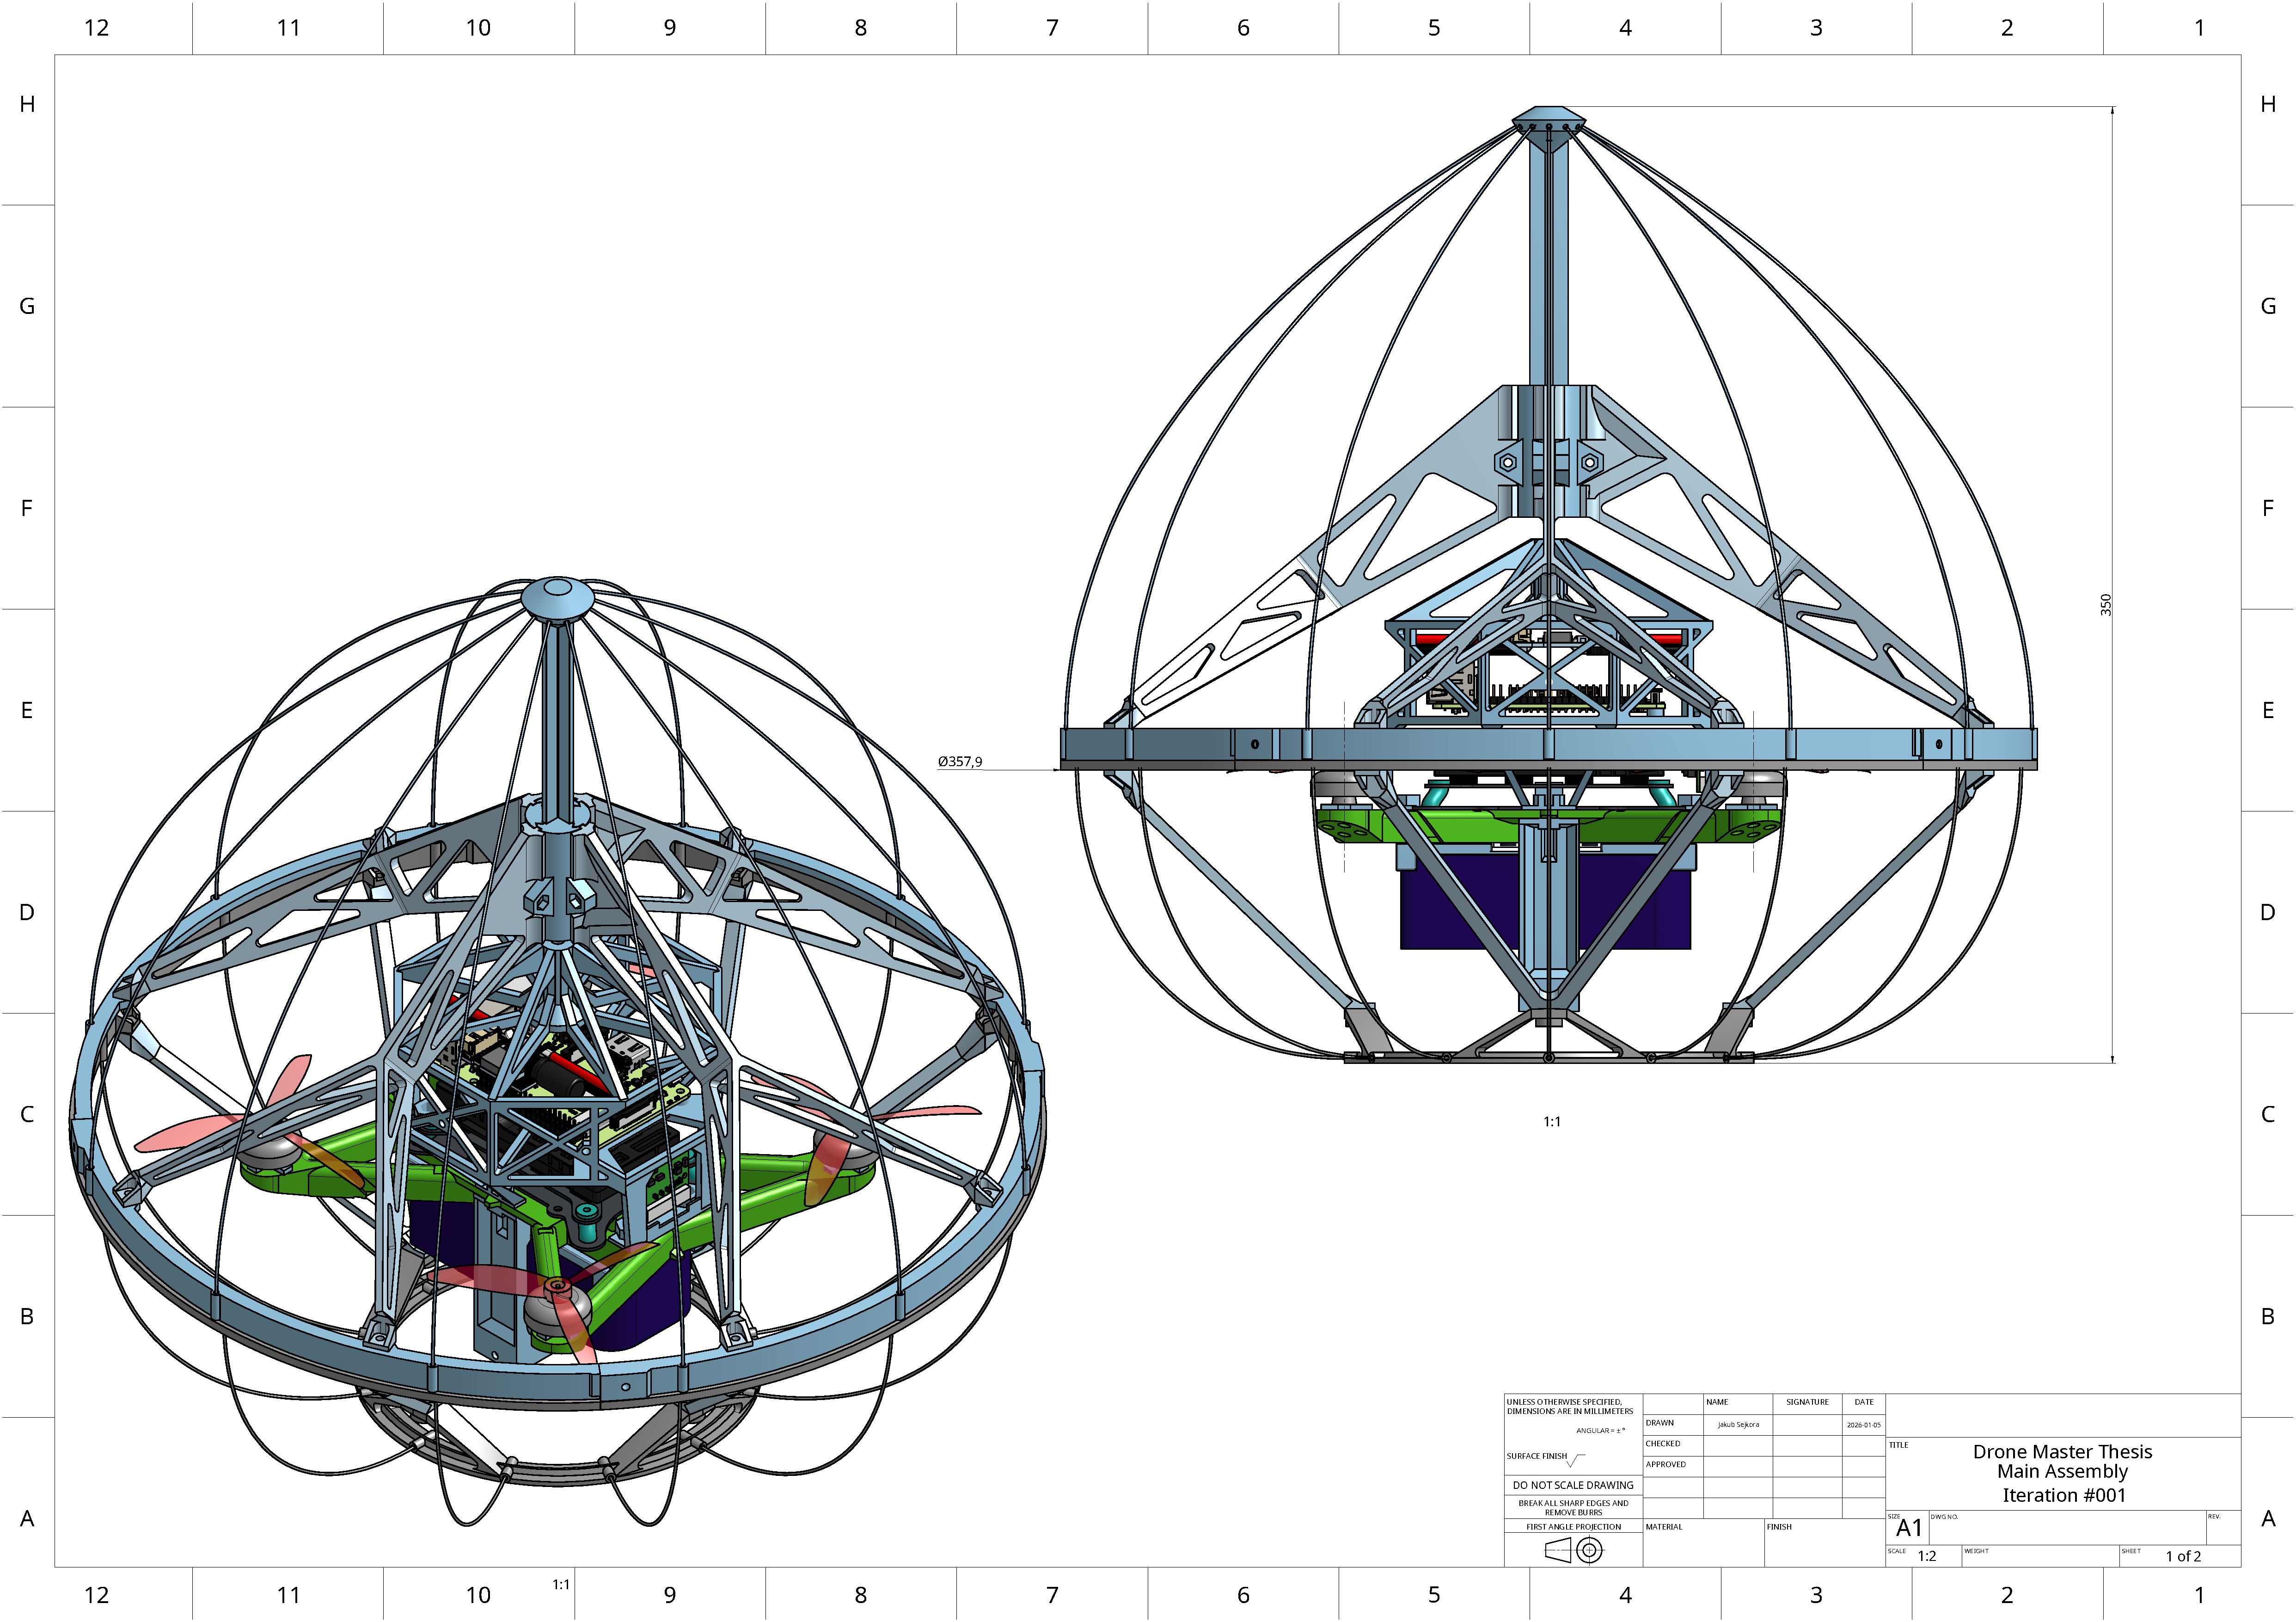
\includegraphics[width=\textwidth,height=0.90\textheight,keepaspectratio]{diagrams/drone_dwg.pdf}
    \caption{Full drone assembly drawing (sheet 1 of 2). The A1 original has been scaled to fit A4 page dimensions.}
    \label{fig:cad_assembly}
\end{figure}
\end{landscape}

\clearpage
\begin{center}
    \vspace*{4cm}
    {\LARGE\textbf{3D CAD Model}} \\[2em]
    \qrcode[height=4cm]{https://cad.onshape.com/documents/7cbebd1596e6b9c6c98f0e3f/w/5e6908f6b6eb3e1d2b683876/e/866a8eb8a37ae0706272cbd1?renderMode=0&uiState=6a4263881140b20f69c49cb9} \\[1em]
    {\footnotesize\url{https://cad.onshape.com/documents/7cbebd1596e6b9c6c98f0e3f/w/5e6908f6b6eb3e1d2b683876/e/866a8eb8a37ae0706272cbd1?renderMode=0\&uiState=6a4263881140b20f69c49cb9}} \\[2em]
    \large{The complete drone assembly CAD model, including the frame, protective cage, and all mounted components. This OnShape document served as the primary mechanical reference throughout the design, manufacturing, and assembly phases.}
    \vfill
\end{center}

\endinput

\section{EXAMPLE Figures}

The ``\verb|figure|'' environment should be used for figures. One or
more images can be placed within a figure. If your figure contains
third-party material, you must clearly identify it as such, as shown
in the example below.

\begin{figure}[h]
\centering
\includegraphics[width=1\linewidth]{Figures/MyriadX.png}
\caption{Diagram of the Intel Movidius Myriad X architecture. \cite{myriadxfigure}}
\label{fig:myriadx}
\end{figure}

Your figures should contain a caption which describes the figure to
the reader.

Figure captions are placed {\itshape below} the figure.
\section{Tables}

The experimental results are summarized in the following tables. These
present aggregated metrics across the fixed and rotating cage configurations
for each incidence angle tested.

\begin{table}[htbp]
  \centering
  \caption{Experiment configurations tested}
  \label{tab:experiment_configs}
  \begin{tabular}{ccl}
    \toprule
    Incidence Angle & Cage Type & Valid Passes \\
    \midrule
    $30^\circ$ & Fixed & $N$ \\
    $30^\circ$ & Rotating & $N$ \\
    $45^\circ$ & Fixed & $N$ \\
    $45^\circ$ & Rotating & $N$ \\
    $60^\circ$ & Fixed & $N$ \\
    $60^\circ$ & Rotating & $N$ \\
    $75^\circ$ & Fixed & $N$ \\
    $75^\circ$ & Rotating & $N$ \\
    \bottomrule
  \end{tabular}
\end{table}

\section{Mathematics}

This thesis uses standard mathematical notation for rigid-body dynamics and
control theory. Key symbols and conventions are defined here for reference.

\subsection{Coordinate Frames}

The drone's pose is expressed in two coordinate frames:
\begin{itemize}
    \item \textbf{World frame (ENU):} $X$ east, $Y$ north, $Z$ up.
    \item \textbf{Body frame:} $x_b$ forward, $y_b$ right, $z_b$ down
    (NED convention per PX4 firmware).
\end{itemize}

Position is denoted $\mathbf{p} = [x, y, z]^\mathsf{T}$,
velocity $\mathbf{v} = [v_x, v_y, v_z]^\mathsf{T}$, and
acceleration $\mathbf{a} = [a_x, a_y, a_z]^\mathsf{T}$.

\subsection{Drone Dynamics}

The quadcopter's rotational dynamics are governed by the Euler equations:

\begin{equation}
    \mathbf{I} \dot{\boldsymbol{\omega}} + \boldsymbol{\omega} \times (\mathbf{I} \boldsymbol{\omega}) = \boldsymbol{\tau}
\end{equation}

where $\mathbf{I}$ is the inertia tensor, $\boldsymbol{\omega}$ the angular velocity,
and $\boldsymbol{\tau}$ the applied torque from motor thrust differentials.

\subsection{Collision Kinematics}

Impact deceleration is measured as the peak magnitude of the IMU acceleration vector
during the collision window:

\begin{equation}
    \|\mathbf{a}_{\text{peak}}\| = \max_{t \in T_{\text{collision}}} \sqrt{a_x(t)^2 + a_y(t)^2 + a_z(t)^2}
\end{equation}

This is reported in multiples of standard gravity $g = 9.81\ \text{m}\,\text{s}^{-2}$.


\newpage
\bibliographystyle{plainnat}
\bibliography{IEEEabrv,references,references_non_zotero}
% \bibliographystyle{IEEEtran}

%\clearpage

%\listoffigures

%\clearpage

%\listoftables

%\clearpage

%\listoflistings

\end{document}